% Compiler: pdfLaTeX. BibTeX is run automatically by Overleaf/latexmk.
\documentclass[11pt,a4paper]{article}
\usepackage[T1]{fontenc}
\usepackage[utf8]{inputenc}
\usepackage{lmodern,microtype}
\usepackage[margin=25mm,headheight=14pt]{geometry}
\usepackage{amsmath,amssymb}
\usepackage{booktabs,longtable,array,ragged2e}
\usepackage{caption}
\captionsetup{font=small,labelfont=bf,justification=justified,singlelinecheck=false}
\usepackage{tikz,pgfplots}
\usetikzlibrary{arrows.meta,positioning,calc}
\usepgfplotslibrary{groupplots,statistics,colormaps}
\pgfplotsset{compat=1.18,every axis/.append style={font=\footnotesize,label style={font=\footnotesize},tick label style={font=\scriptsize},legend style={font=\scriptsize,draw=none},axis lines=left,grid=major,grid style={gray!18},legend cell align=left},colormap={diverging}{rgb255(0cm)=(33,102,172);rgb255(1cm)=(247,247,247);rgb255(2cm)=(178,24,43)}}
\usepackage[numbers,sort&compress]{natbib}
\usepackage{xurl}
\usepackage[hidelinks,bookmarksnumbered]{hyperref}
\usepackage{bookmark}
\usepackage[section]{placeins}
\usepackage{fancyvrb,fvextra}
\usepackage{fancyhdr}
\pagestyle{fancy}\fancyhf{}
\fancyhead[L]{\small ML-TradeEngine research}
\fancyhead[R]{\small Historical study; prospective interim}
\fancyfoot[C]{\thepage}
\renewcommand{\headrulewidth}{0.3pt}
\setlength{\parindent}{1.3em}\setlength{\parskip}{2pt}
\setlength{\emergencystretch}{2em}
\raggedbottom
\renewcommand{\topfraction}{.9}
\renewcommand{\bottomfraction}{.85}
\renewcommand{\textfraction}{.08}
\renewcommand{\floatpagefraction}{.65}
\clubpenalty=10000\widowpenalty=10000
\setcounter{tocdepth}{2}
\hypersetup{pdftitle={Causal Forecasts, Constrained Portfolios, and Prospective Operation},pdfauthor={Yash Kataria}}
\begin{document}
\pagenumbering{roman}
\begin{titlepage}
\centering
\vspace*{8mm}
{\LARGE\bfseries Causal Forecasts, Constrained Portfolios, and Prospective Operation\par}
\vspace{5mm}
{\large An auditable empirical study of ML-TradeEngine\par}
\vspace{8mm}
{\Large Yash Kataria\par}
\vspace{6mm}
{28 September 2026\par}
\vspace{6mm}
{\small Historical evidence through 25 September 2026.\\Prospective sections remain interim; external broker orders are disabled.\par}
\vspace{10mm}
\begin{minipage}{.94\textwidth}
\section*{Abstract}
We evaluate causal probabilistic forecasts and capital-constrained local execution using 22 equities and ETFs, preserved historical snapshots, controlled chronological refits and a separately frozen prospective collector. The saved experiment supplies 15,092 instrument-date decisions from 726 rolling refits. In its consumed recent audit, the calibrated mixture has 37.59\% accuracy and 1.0882 log loss, compared with 40.62\% and 1.0756 for the trailing prior. Its paired log-loss disadvantage is 0.0126, with a date-block 95\% interval [-0.0025, 0.0269]. Fresh-capital audit accounts return -0.46\% for the adaptive hybrid and 2.55\% for the matched equal-weight control after costs. The follow-up executes 848 registered training trials, with feature, calibration, adaptation and held-instrument comparisons. The product includes a sealed local collector, persistent ledgers and a session-aware schedule; engineering evidence is scoped separately from trading superiority. These experiments do not establish a defensible deployable edge. Historical analyses are exploratory, prospective sections remain interim, and external broker orders remain disabled.

\par\medskip
\noindent\textbf{Keywords:} quantitative trading; probability calibration; walk-forward evaluation; dependent-sample inference; paper trading; reproducibility.
\end{minipage}
\vfill
{\small Research report. Journal-specific formatting can be applied when a publication venue is selected.\par}
\end{titlepage}
\setcounter{page}{2}
\tableofcontents
\clearpage
\pagenumbering{arabic}

\section{Motivation and research questions}\label{sec:section-01}

A trading research system must answer two questions that are easy to confuse: whether its calculations represent the stated strategy, and whether that strategy has useful economic performance. Correct accounting is necessary for the second question, but it cannot answer it. Likewise, a profitable curve cannot validate data that were unavailable at the simulated decision time. This study follows the entire chain from public observations to predictions, constrained targets, simulated fills, persisted account state and research claims. The output is an executable local paper-trading product and a versioned empirical record. No external broker execution is part of the experiment.

The starting repository contained classifiers, a strategy zoo, an ensemble, a dashboard and saved backtests. Earlier audits identified accounting and timing defects. Subsequent repairs produced a sealed adaptive experiment and a short technical report. We preserve that experiment and examine its full prediction and ledger records instead of inferring behavior from headline accuracy or isolated screenshots. This follow-up adds class and instrument diagnostics, controlled refits, transfer tests, execution sensitivities and operational evidence. Previously inspected historical observations are explicitly exploratory. A new analysis of an old holdout does not restore its independence.

Our first question is whether causal forecasts improve probability quality and directional classification over a trailing class-frequency estimate and simple forecasting controls. The primary predictive endpoint is the paired, date-averaged log-loss difference against the prior. Accuracy, balanced accuracy, class F1 and multiclass Brier score explain different aspects of the result. A correct class prediction and a profitable trade are separate events, so no accuracy threshold is used as a proof of alpha.

The second question is whether a hybrid adds net economic value over its components and comparable simple policies when every strategy must finance its holdings through one account. The primary economic endpoint is the daily net-return difference from a costed, risk-constrained equal-weight account on matching dates. We distinguish this account from a descriptive frictionless SPY reference. The third question concerns where errors occur: classes, instruments, calendar blocks, observed volatility conditions, disagreement between experts and confident mistakes. Such conditional descriptions identify hypotheses; they do not by themselves establish a causal mechanism.

The fourth question is sensitivity to features, calibration, gate construction, training history, refit cadence and execution assumptions. Controlled comparisons change a specified factor while preserving the eligible information set and outcome definition. The fifth question concerns operation: whether the same policy can run from fresh inputs with persistent capital, restart after faults, refuse invalid state and produce durable evidence on its registered schedule. These questions define separate engineering, historical-evidence, prospective-operation and manuscript decisions. Broker readiness is a further decision outside the authorized scope.

\section{Related work and the scope of comparison}\label{sec:section-02}

Machine learning can model nonlinear conditional relationships in asset returns. Gu, Kelly and Xiu compare a broad range of methods for risk-premium prediction and examine the importance of interactions \citep{gu2020}. Their result motivates careful predictive comparisons; it does not supply a performance target for this project. Their universe, prediction horizon, information set and portfolio construction differ from our small daily classification study. We do not copy their reported economic gains into a benchmark table or interpret a different task as a replication.

A simple trend rule is a demanding control for a more elaborate trading architecture because it can capture persistent price behavior without learning a high-dimensional decision boundary. Time-series momentum has been studied across futures markets \citep{momentum2012}. Our rule combines a trailing price-average condition with intermediate-horizon momentum on the existing equity/ETF universe. It is long-only and financed through the same constrained local ledger as the ML policy. It is therefore a project control inspired by trend-following, not a reproduction of the published futures strategy.

Gradient boosting provides a flexible additive model built through successive loss reduction \citep{friedman2001}. We pair a shallow histogram boosting classifier with regularized multinomial logistic regression to contrast nonlinear and linear decision surfaces. The logistic model is both a component and a useful simplicity control. Fixed capacity and chronological fitting make the comparison interpretable. Increasing model count or training duration after seeing poor outer-period results would change the scientific question and enlarge the search history; it would not repair a failed hypothesis.

Probability forecasts require more than class ranking. Proper scoring rules reward distributions that represent the forecaster's uncertainty \citep{gneiting2007}. Log loss penalizes confident wrong answers strongly, whereas accuracy only considers the largest probability. The Brier score measures squared error across the complete class distribution. Temperature scaling is a low-dimensional way to alter sharpness while preserving each row's ordering \citep{guo2017}. Evidence from other application domains does not imply that temperature scaling must improve financial forecasts. We therefore compare raw and calibrated mixtures on identical outer observations and disclose the samples used to fit the temperature.

Dependent observations complicate uncertainty. Adjacent forward-return labels overlap, and symbols respond to common market shocks. Resampling instrument-date rows independently would overstate the effective sample size. Block resampling follows the general motivation of dependent-data bootstrap methods \citep{kunsch1989}, while HAC estimators provide a complementary approach for autocorrelated averages \citep{newey1987}. Our implementation preserves the entire cross section within a sampled date and examines several block lengths. The assumptions remain approximate when the return-generating process shifts over time.

Multiple testing is especially consequential in strategy research. Financial factor evidence illustrates how an extensive search can make conventional single-test thresholds misleading \citep{harvey2016}. Holm adjustment controls a declared family of comparisons \citep{holm1979}, but no adjustment can recover undocumented researcher choices. The Deflated Sharpe Ratio and probability-of-backtest-overfitting literature address aspects of selection risk \citep{bailey2014,bailey2015}. We do not report those estimators here because a complete comparable trial history and their required assumptions are not available. The current registry makes the new comparison family explicit; it does not erase earlier exposure.

Covariance shrinkage is motivated by the instability of estimated risk matrices \citep{ledoit2004}. Our risk rule uses a fixed blend of sample covariance and its diagonal. This is a transparent regularization assumption, not an implementation of the cited paper's optimal shrinkage estimator. Exchange timing follows the official NYSE calendar \citep{nyse2026}. The operational design also recognizes that a scheduled workflow file does not guarantee execution; workflow failures require direct evidence \citep{github2026}. These references establish methods and constraints. All empirical performance claims below come from this project's saved or newly executed experiments.

\section{Data, availability and evidence accounting}\label{sec:section-03}

\subsection{Universe and provider snapshots}

The verified market panel contains 55,242 instrument-session observations on 2,511 common market dates. There are 686 recorded decision dates, 680 with mature outcomes, and 132 instrument-date predictions whose outcomes are unavailable at the historical cutoff. The inherited release reports 726 refits. The inventory rechecked 722 preserved files and directly compared 66 saved reproduction outputs. These are new integrity checks of saved records, not a claim that all old models were trained again.

The universe was inherited from the project rather than sampled from historical index constituents. It mixes individual surviving companies, broad-market funds, sector funds and alternative-asset funds. Economic exposures overlap: holding a growth stock and a fund that contains it does not create two independent bets. The declared growth-group limit captures only one part of that overlap. We cannot estimate delisting bias from this universe, and we do not interpret the results as a market-wide stock-selection claim.

Raw provider OHLCV and adjusted series are separate artifacts. The term raw refers to the provider's returned fields before this pipeline's adjustment transformation; it does not certify an archival, unadjusted exchange tape. Adjusted prices incorporate the vendor's present interpretation of splits and distributions. Each snapshot records retrieval time and hashes. Historical availability uses an explicit completed-session convention because the provider does not supply an immutable historical arrival timestamp for every bar. A current-vintage reconstruction is not equivalent to a point-in-time archive.

For the local simulation, quantities are total-return proxy units. Future provider revisions can rescale historical adjusted prices, so daily marks chain the newly observed adjusted return onto stored marks. That convention avoids treating a uniform rescaling as a windfall or loss in existing holdings. It does not implement broker shares, dividend cash payments, fractional-share restrictions or corporate-action entitlements. Raw responses and available action events are retained for provenance, while broker accounting remains a separate unimplemented contract.

\noindent Table~\ref{tab:1} reports dataset flow; counts are instrument-dates unless the stage explicitly says dates.

\begin{table}[!htbp]\centering\footnotesize\setlength{\tabcolsep}{3pt}\renewcommand{\arraystretch}{1.14}
\caption{Dataset flow; counts are instrument-dates unless the stage explicitly says dates}\label{tab:1}
\begin{tabular}{@{}>{\raggedright\arraybackslash}p{\dimexpr 0.82819\textwidth-3.000pt\relax}>{\raggedleft\arraybackslash}p{\dimexpr 0.17181\textwidth-3.000pt\relax}@{}}
\toprule
\textbf{Stage} & \textbf{Count} \\
\midrule
raw\_\allowbreak{}symbol\_\allowbreak{}sessions & 55,242 \\
common\_\allowbreak{}market\_\allowbreak{}dates & 2,511 \\
feature\_\allowbreak{}complete\_\allowbreak{}symbol\_\allowbreak{}sessions & 49,698 \\
warmup\_\allowbreak{}symbol\_\allowbreak{}sessions & 5,544 \\
pre\_\allowbreak{}evaluation\_\allowbreak{}feature\_\allowbreak{}complete\_\allowbreak{}symbol\_\allowbreak{}sessions & 34,606 \\
decision\_\allowbreak{}symbol\_\allowbreak{}sessions & 15,092 \\
mature\_\allowbreak{}labeled\_\allowbreak{}symbol\_\allowbreak{}sessions & 14,960 \\
unmatured\_\allowbreak{}symbol\_\allowbreak{}sessions & 132 \\
\bottomrule\end{tabular}\par\smallskip
\raggedright\textit{Source:} \path{data/research-v2/tables/diag_dataset_flow.csv}.
\end{table}


\noindent Figure~\ref{fig:1} shows coverage, retained observations and class support from the saved panel.

\begin{figure}[htbp]\centering
% Native editable figure; frozen statistics 0d291b4aebf8c524dc6705d872c070feb990e86a1cebbd59a758f400b240c952
\begin{minipage}[t]{.48\linewidth}\centering
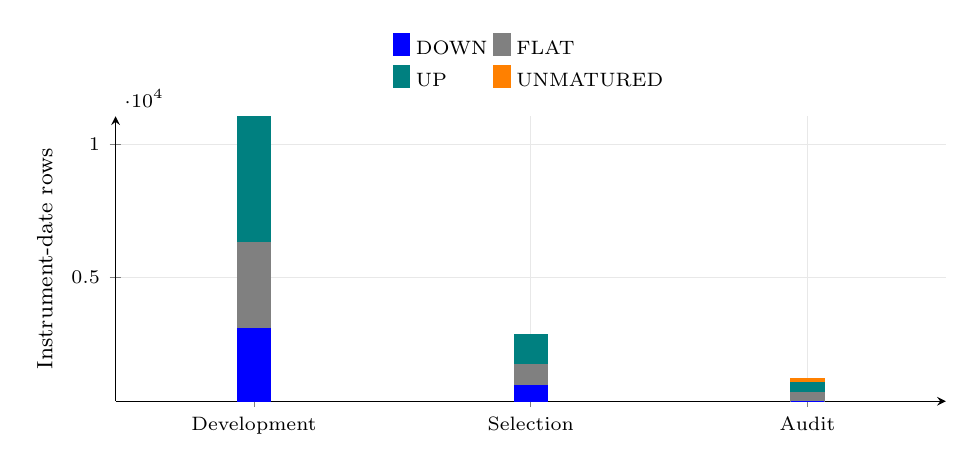
\begin{tikzpicture}
\begin{axis}[width=\linewidth,height=5.2cm,ybar stacked,bar width=12pt,xtick={0,1,2},xticklabels={Development,Selection,Audit},ylabel={Instrument-date rows},legend columns=2,legend style={at={(0.5,1.05)},anchor=south},enlarge x limits=.25]
\addplot+[blue,fill=blue,draw=blue] coordinates {(0,3081) (1,952) (2,351)};
\addlegendentry{DOWN}
\addplot+[gray,fill=gray,draw=gray] coordinates {(0,3230) (1,768) (2,326)};
\addlegendentry{FLAT}
\addplot+[teal,fill=teal,draw=teal] coordinates {(0,4733) (1,1140) (2,379)};
\addlegendentry{UP}
\addplot+[orange,fill=orange,draw=orange] coordinates {(0,0) (1,0) (2,132)};
\addlegendentry{UNMATURED}

\end{axis}
\end{tikzpicture}
\end{minipage}
\hfill
\begin{minipage}[t]{.48\linewidth}\centering
\resizebox{\linewidth}{!}{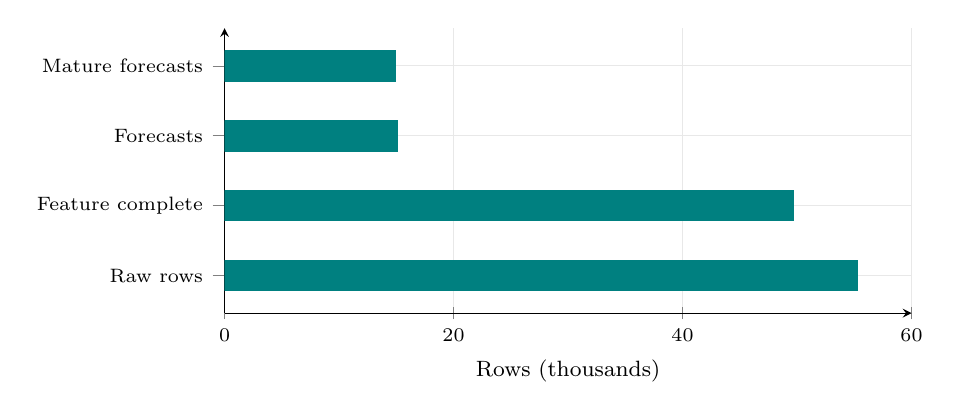
\begin{tikzpicture}
\begin{axis}[width=.85\linewidth,height=5.2cm,xbar,bar width=11pt,ytick={0,1,2,3},yticklabels={Raw rows,Feature complete,Forecasts,Mature forecasts},xlabel={Rows (thousands)},enlarge y limits=.18,xtick={0,20000,40000,60000},xticklabels={0,20,40,60},xmax=60000,scaled x ticks=false,x tick label style={/pgf/number format/fixed},xmin=0]
\addplot+[teal] coordinates {(55242,0) (49698,1) (15092,2) (14960,3)};
\end{axis}
\end{tikzpicture}
}\end{minipage}
\caption{Coverage, retained observations and class support from the saved panel.}\label{fig:1}
\end{figure}

\subsection{Admission, missingness and labels}

Every admitted price panel must have unique, monotonically ordered session keys, finite positive OHLC values, valid high/low ranges and positive observed volume. The exchange calendar, rather than a generic weekday index, defines expected sessions. There is no holiday padding, synthetic zero-volume bar, stale-price forward fill or silent fallback to the last successful forecast. An unavailable bar stops the applicable batch before account decisions. Dropping a record, skipping an event and predicting FLAT are different states and remain distinguishable in the evidence.

For information observed at the end of session t, the first modeled fill is the next completed close. The target return is therefore:

\begin{equation}\label{eq:target}r^{\mathrm{target}}_t=\frac{C_{t+6}}{C_{t+1}}-1.\end{equation}

A return below -1\% is DOWN, above +1\% is UP, and an observed return between those thresholds is FLAT. A target whose ending close has not occurred is unobserved, not FLAT. Strict fitting eligibility requires its endpoint to precede the refit decision. The distinction matters twice: at the tail of the study, where decisions outnumber mature labels, and at partition boundaries, where adjacent labels can otherwise reveal later evaluation prices.

Dataset accounting is performed separately for price rows, usable feature rows, decision rows, label-complete instrument-dates and account sessions. A portfolio needs marks even when an outcome label is not yet mature. Thus the last account sessions legitimately contribute to equity measurement while being excluded from classification. The tables and claim map preserve those denominators instead of calling every row a sample with independent statistical information.

\subsection{Exposure log and optional information}

All historical dates inspected in the prior tasks or saved release are listed in the evaluation-exposure log. The old development, selection and audit labels are retained as names for reproducible date ranges, not as a claim that the current analyst is blind to them. The new controlled experiments use development-era chronological blocks and do not replace the previously selected prospective shadow. Historical results are useful for diagnosing a design and measuring its behavior; independent confirmation must come from later observations under a frozen rule.

Macro, news and crypto are excluded from the primary information set. A working public endpoint does not establish historical vintage eligibility. Revised macro observations need release/vintage timestamps; news requires retained content, version and availability times; a bounded recent crypto endpoint does not supply the requested long archive. Legacy XGB, LGBM, LSTM, MoE and zoo outputs remain preserved. Their different targets, information sets and splits prevent treating their old headline scores as controlled architectural comparisons. The registry records scope exclusions rather than silently dropping weak models.

\section{Methods and the shared execution contract}\label{sec:section-04}

\subsection{Features and forecasting models}

\noindent Table~\ref{tab:2} reports feature definitions and information availability.

\begin{table}[!htbp]\centering\footnotesize\setlength{\tabcolsep}{3pt}\renewcommand{\arraystretch}{1.14}
\caption{Feature definitions and information availability}\label{tab:2}
\begin{tabular}{@{}>{\raggedright\arraybackslash}p{\dimexpr 0.15306\textwidth-4.000pt\relax}>{\raggedright\arraybackslash}p{\dimexpr 0.43878\textwidth-4.000pt\relax}>{\raggedright\arraybackslash}p{\dimexpr 0.40816\textwidth-4.000pt\relax}@{}}
\toprule
\textbf{Family} & \textbf{Definition} & \textbf{Availability} \\
\midrule
Returns & Close /\allowbreak{} lagged close - 1 & Trailing 1, 5, 21, 63, 126, 252 sessions \\
Volatility & Sample standard deviation of daily return & Trailing 21 /\allowbreak{} 63 sessions \\
Relative return & Instrument return minus SPY return & Trailing 21 /\allowbreak{} 63 sessions \\
Trend & Close /\allowbreak{} moving mean - 1 & Trailing 20 /\allowbreak{} 50 /\allowbreak{} 200 sessions \\
Gap /\allowbreak{} range & Open /\allowbreak{} previous close - 1; (High-Low)/\allowbreak{}Close & Completed current session \\
Volume & Volume /\allowbreak{} trailing mean - 1 & Trailing 20 sessions \\
Momentum & Close lag21 /\allowbreak{} Close lag252 - 1 & Previous completed observations \\
\bottomrule\end{tabular}\par\smallskip
\raggedright\textit{Source:} \path{src/models/adaptive.py::features; research_v2/experiments.py::FAMILIES}.
\end{table}


\noindent Table~\ref{tab:3} reports fixed model configurations and distinct chronological contracts.

\begin{table}[!htbp]\centering\footnotesize\setlength{\tabcolsep}{3pt}\renewcommand{\arraystretch}{1.14}
\caption{Fixed model configurations and distinct chronological contracts}\label{tab:3}
\begin{tabular}{@{}>{\raggedright\arraybackslash}p{\dimexpr 0.23009\textwidth-4.000pt\relax}>{\raggedright\arraybackslash}p{\dimexpr 0.26549\textwidth-4.000pt\relax}>{\raggedright\arraybackslash}p{\dimexpr 0.50442\textwidth-4.000pt\relax}@{}}
\toprule
\textbf{Contract} & \textbf{Component} & \textbf{Configuration} \\
\midrule
Controlled & Hist\allowbreak{}Gradient\allowbreak{}Boosting\allowbreak{}Classifier & max\_\allowbreak{}iter=100; max\_\allowbreak{}leaf\_\allowbreak{}nodes=7; l2\_\allowbreak{}regularization=10; learning\_\allowbreak{}rate=0.05; min\_\allowbreak{}samples\_\allowbreak{}leaf=40; early\_\allowbreak{}stopping=False; random\_\allowbreak{}state=cfg.seed \\
Controlled & LogisticRegression & C=0.1; max\_\allowbreak{}iter=500; random\_\allowbreak{}state=cfg.seed \\
Historical /\allowbreak{} carried pilot & Hist\allowbreak{}Gradient\allowbreak{}Boosting\allowbreak{}Classifier & max\_\allowbreak{}iter=100; max\_\allowbreak{}leaf\_\allowbreak{}nodes=7; l2\_\allowbreak{}regularization=10; learning\_\allowbreak{}rate=0.05; min\_\allowbreak{}samples\_\allowbreak{}leaf=40; early\_\allowbreak{}stopping=False; random\_\allowbreak{}state=cfg.seed \\
Historical /\allowbreak{} carried pilot & LogisticRegression & C=0.1; max\_\allowbreak{}iter=500; random\_\allowbreak{}state=cfg.seed \\
Controlled base & Chronology & history=1008; calibration=63; gate=63; cadence=63 \\
Historical /\allowbreak{} pilot & Chronology & window=1008; calibration=126; min\_\allowbreak{}fit=504; retrain\_\allowbreak{}every=21 \\
Both & Temperature candidates & [0.75, 1, 1.5, 2, 3] \\
\bottomrule\end{tabular}\par\smallskip
\raggedright\textit{Source:} \path{data/research-v2/tables/model_configurations.csv; evidence/configuration-sources.json}.
\end{table}


The scale-free feature set combines trailing returns, volatility, prices relative to moving averages, market-relative returns, intraday range, overnight gap, volume ratio and intermediate-horizon momentum. Rolling operations use only the observed prefix. There is no full-sample normalization or learned feature screening outside the fitting partition. The logistic scaler is fitted on eligible fitting rows and then applied unchanged to calibration and evaluation. Feature order is part of the inference schema; matching names in a different order is insufficient.

The logistic expert minimizes regularized multinomial cross-entropy. The tree expert fits shallow histogram-based boosting with fixed iteration count, leaf budget and regularization. Their raw mixture is the arithmetic mean of their probability vectors. Temperature scaling applies:

\begin{equation}\label{eq:temperature}p_T(c\mid x)=\frac{\exp\{\log p_{\mathrm{raw}}(c\mid x)/T\}}{\sum_k\exp\{\log p_{\mathrm{raw}}(k\mid x)/T\}}.\end{equation}

The temperature is selected only from its registered candidate set using eligible past calibration labels. Because this transformation preserves class ordering, its direct purpose is probability quality rather than creating a different argmax classification. The training-frequency control uses Laplace-smoothed class counts from the fitting sample. Always-UP is a directional control; its near-deterministic probabilities make it a poor probability benchmark when another class occurs, which is why the prior is primary for log loss.

The sealed release calibrated temperature and estimated gate benefit on the same trailing block. That is chronologically causal but permits internal optimism from evaluating a selected temperature on its fitting block. The follow-up separates fitting, temperature selection and gate evaluation with endpoint-based purges. This experiment asks whether the gate's apparent past advantage survives a distinct eligible block. It does not assume that separating the blocks must improve returns; fewer calibration or gate observations may increase estimation variance.

\subsection{Chronology, folds and refitting}

\noindent Figure~\ref{fig:2} shows architecture of the isolated collection and research paths.

\begin{figure}[htbp]\centering
% Native editable figure; frozen statistics 0d291b4aebf8c524dc6705d872c070feb990e86a1cebbd59a758f400b240c952
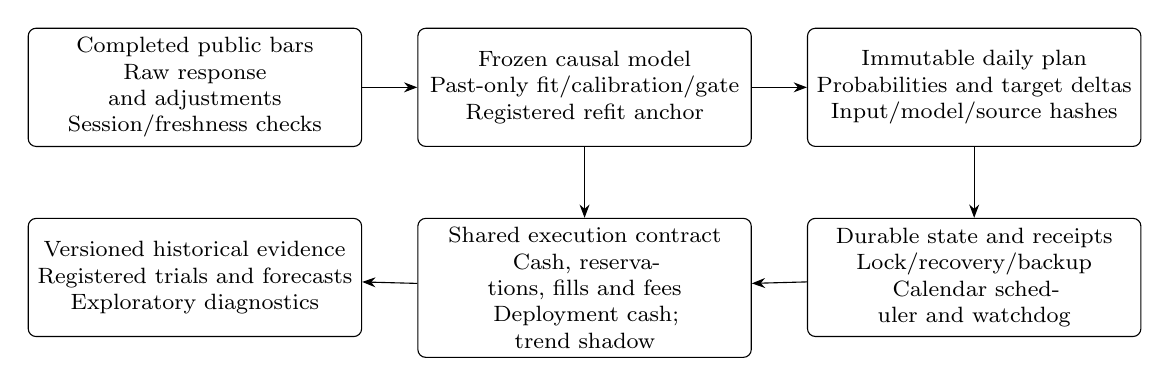
\begin{tikzpicture}[node distance=9mm and 7mm,box/.style={draw,rounded corners=1mm,align=center,text width=40mm,minimum height=15mm,font=\footnotesize},>=Stealth]
\node[box] (data) {Completed public bars\\Raw response and adjustments\\Session/freshness checks};
\node[box,right=of data] (model) {Frozen causal model\\Past-only fit/calibration/gate\\Registered refit anchor};
\node[box,right=of model] (plan) {Immutable daily plan\\Probabilities and target deltas\\Input/model/source hashes};
\node[box,below=of data] (research) {Versioned historical evidence\\Registered trials and forecasts\\Exploratory diagnostics};
\node[box,below=of model] (account) {Shared execution contract\\Cash, reservations, fills and fees\\Deployment cash; trend shadow};
\node[box,below=of plan] (state) {Durable state and receipts\\Lock/recovery/backup\\Calendar scheduler and watchdog};
\draw[->] (data)--(model);\draw[->] (model)--(plan);\draw[->] (plan)--(state);\draw[->] (model)--(account);\draw[->] (state)--(account);\draw[->] (account)--(research);
\end{tikzpicture}
\caption{Architecture of the isolated collection and research paths.}\label{fig:2}
\end{figure}

\noindent Figure~\ref{fig:3} shows information, fill and label availability under the execution-aligned target.

\begin{figure}[htbp]\centering
% Native editable figure; frozen statistics 0d291b4aebf8c524dc6705d872c070feb990e86a1cebbd59a758f400b240c952
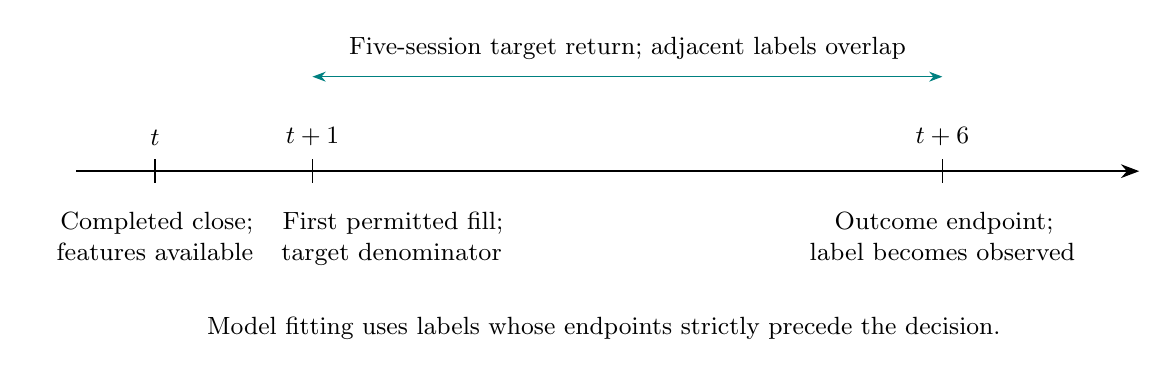
\begin{tikzpicture}[x=1cm,y=1cm,>=Stealth,font=\small]
\draw[->,thick] (0,0)--(13.5,0);
\foreach \x/\t in {1/t,3/{t+1},11/{t+6}}{\draw (\x,-.15)--(\x,.15);\node[above] at (\x,.2) {$\t$};}
\node[align=center,text width=30mm,below] at (1,-.4) {Completed close;\\features available};
\node[align=center,text width=33mm,below] at (4,-.4) {First permitted fill;\\target denominator};
\node[align=center,text width=38mm,below] at (11,-.4) {Outcome endpoint;\\label becomes observed};
\draw[<->,teal] (3,1.2)--(11,1.2);\node[above] at (7,1.3) {Five-session target return; adjacent labels overlap};
\node[align=center] at (6.7,-2.0) {Model fitting uses labels whose endpoints strictly precede the decision.};
\end{tikzpicture}
\caption{Information, fill and label availability under the execution-aligned target.}\label{fig:3}
\end{figure}

At a refit decision, eligible labels are determined by their actual session endpoints. Fitting, calibration and gate partitions are chronological. Purging removes any earlier-partition target whose outcome reaches the next partition's first decision. This rule is derived from execution timing rather than a conveniently chosen gap. A transform learned from a preceding partition is applied to later partitions without refitting. All fold records retain first/last dates, label endpoints, sample counts and source/configuration hashes.

The controlled outer dates comprise four disjoint blocks, each containing the first 63 sessions of a development half-year. Date-block resampling stays within each outer block. The bounded experiment design varies one registered factor at a time. There is no Cartesian hyperparameter search. If an inner choice is fitted, that choice is made entirely before its outer block; outer results never select a replacement pilot policy. Training-history and refit-cadence experiments align features, targets and evaluation dates, preventing a model trained on a different information set from masquerading as evidence about architecture. Additional seeds cover six representative instruments; they do not cover every instrument. Registered seeds characterize estimator variability separately from uncertainty across dates. Seeds and correlated instruments are not independent replications of the market.

The operational contract has an explicit exchange-session refit anchor and an explicit startup model. Research replay and the daily runner use the same anchor. Weekly target changes occur on the last eligible exchange session of the week, including holiday weeks, with an initial allocation decision. Other sessions process pending fills, marks and drawdown controls without routine rebalancing. These v2 rules are versioned changes; they do not retroactively alter the sealed experiment's dates or Friday-only results.

\subsection{From probabilities to constrained targets}

Expected target return is the probability-weighted mean of the fitting sample's class-conditional target returns. A positive prediction only requests an allocation when this estimate exceeds the registered round-trip cost hurdle. The trend intent requires a positive price/long-average ratio and positive intermediate-horizon momentum. A fixed hybrid combines the two intents; the adaptive hybrid allows the ML contribution only when the past-data gate accepts it. The forecasting mixture and the trading hybrid are distinct objects and are named separately in the result tables.

Before account submission, target weights pass long-only, per-instrument, gross and group caps. Trailing covariance is estimated from eligible observed returns, annualized, and shrunk halfway toward its diagonal. If estimated target volatility exceeds the registered cap, all risky target weights are scaled down proportionally. This rule does not guarantee future volatility or drawdown, and estimation error remains visible in sensitivity tests. Idle cash earns zero under the simulated account contract.

Orders represent changes from current holdings toward target holdings, not repeated purchases for repeated UP signals. Pending buys reserve cash; pending sales are not spendable buying power. Orders can be rejected when a price gap exceeds the reserved budget or projected exposure violates limits. A drawdown halt requests reductions and persists through restart. Marked market drift can temporarily breach a target cap between decisions, so the system records a breach and blocks risk-increasing orders rather than pretending a target limit is a pathwise guarantee.

The balance identity is:

\begin{equation}\label{eq:equity}E_t=B_t+\sum_s q_{s,t}M_{s,t},\end{equation}\noindent where $E_t$ is equity, $B_t$ is cash, $q_{s,t}$ is the held quantity and $M_{s,t}$ is the mark for instrument $s$.

Net realized trade profit includes both entry and exit costs. The simulator applies proportional commission and slippage on each fill. Partial exits allocate the corresponding cost basis; terminal holdings remain marked rather than receiving an invented liquidation. This is one account per policy with fixed initial capital, shared constraints and explicit rejection behavior. Summing independent ticker return curves would describe a different, potentially unfundable strategy.

\subsection{Persisted decisions and operational stages}

The collector validates release, dependencies and state before inference. A decision plan records session, information cutoff, data manifest, model versions, probabilities, targets and marks before account processing. The plan is immutable for that session. Account commits and final receipts are recoverable stages: a restart resumes the same plan and uses event IDs to avoid duplicate fills. Concurrent CLI, dashboard and scheduler requests share the same lock and state owner.

Release/model storage is separate from mutable account state. Backups retain original receipts and database state, and restoration is checked at the recorded original path after moving the original state out of the way. Relocating embedded absolute artifact paths is outside the supported recovery contract. A stale writer, truncated file, missing model or changed source must cause a visible halt; a success-shaped fallback would contaminate both the account and the research dataset. Changes to the collector after qualification require a new release and evidence. The old source and sealed releases are preserved as rollback and historical reproduction assets.

\section{Experimental design, inference and computational budget}\label{sec:section-05}

The controlled study completed 848 registered trials and 1,696 estimator fits, in addition to 4 development runtime-pilot fits. Its base evaluation spans 252 outer dates and 5,544 unique base instrument-date decisions. The registered families contain 17 predictive contrasts and 8 economic contrasts. Repeated model views and seed runs are retained, but never counted as additional independent market observations.

\noindent Table~\ref{tab:4} reports frozen controlled training design.

\begin{table}[!htbp]\centering\footnotesize\setlength{\tabcolsep}{3pt}\renewcommand{\arraystretch}{1.14}
\caption{Frozen controlled training design}\label{tab:4}
\begin{tabular}{@{}>{\raggedright\arraybackslash}p{\dimexpr 0.34646\textwidth-4.800pt\relax}>{\raggedleft\arraybackslash}p{\dimexpr 0.15354\textwidth-4.800pt\relax}>{\raggedleft\arraybackslash}p{\dimexpr 0.15354\textwidth-4.800pt\relax}>{\raggedleft\arraybackslash}p{\dimexpr 0.17323\textwidth-4.800pt\relax}>{\raggedleft\arraybackslash}p{\dimexpr 0.17323\textwidth-4.800pt\relax}@{}}
\toprule
\textbf{Variant} & \textbf{Trials} & \textbf{Targets} & \textbf{Outer folds} & \textbf{Seeds} \\
\midrule
base & 136 & 22 & 4 & 42,137,2026 \\
without\_\allowbreak{}momentum & 88 & 22 & 4 & 42 \\
without\_\allowbreak{}trend & 88 & 22 & 4 & 42 \\
without\_\allowbreak{}risk & 88 & 22 & 4 & 42 \\
without\_\allowbreak{}context\_\allowbreak{}volume & 88 & 22 & 4 & 42 \\
fraction\_\allowbreak{}0.5 & 88 & 22 & 4 & 42 \\
fraction\_\allowbreak{}0.75 & 88 & 22 & 4 & 42 \\
history\_\allowbreak{}504 & 88 & 22 & 4 & 42 \\
cadence\_\allowbreak{}21 & 72 & 6 & 4 & 42 \\
transfer & 24 & 6 & 4 & 42 \\
\bottomrule\end{tabular}\par\smallskip
\raggedright\textit{Source:} \path{data/research-v2/experiments/design.json}.
\end{table}


The primary predictive comparison averages each day's candidate-minus-prior log-loss difference across symbols, then resamples contiguous date blocks. Keeping the cross section intact avoids treating a market-wide error as many independent surprises. Circular wrapping allows every date to start a block, but short samples provide limited distinct market episodes. Block-length sensitivity examines a label-horizon-scale block, the registered primary block and a longer block. Confidence intervals describe the behavior of this historical sample under the resampling assumptions; they do not make the consumed audit confirmatory.

Economic comparisons use identically indexed daily net returns. Rebased charts make date-range returns visually comparable but do not reset account holdings. Where a fresh-capital replay is reported, it explicitly begins a new account and is separately labeled. CAGR compounds the observed return over its annualized duration. The new portfolio diagnostics use a zero risk-free rate for Sharpe and a zero minimum acceptable return for Sortino, consistent with zero-yield cash. The sealed release separately reports Sharpe relative to a fixed annual hurdle; those differently defined values are never interchanged. Sortino uses downside deviation relative to its disclosed target. Undefined zero-variance statistics remain undefined rather than being converted into evidence for a strategy.

Hypothesis families come from registered contrasts. Holm-adjusted values apply separately to the specified predictive and economic families. Additional class, symbol and regime slices are descriptive unless entered into a distinct family before computation. This avoids presenting a favorable post hoc slice as a new independent experiment. Effect sizes and intervals take precedence over binary significance language. Approximate minimum-detectable-effect calculations use the estimated sampling variability; they are design aids, not guarantees of future power.

Execution robustness perturbs clearly named assumptions. Cost changes can retain decisions while changing financing and fills. Delaying execution or restricting fill size may alter exposure and subsequent account behavior. Missing-bar tests are admission/recovery tests and must fail before decisions rather than interpolate a fictional observation. Risk-parameter changes create a different target policy and are classified accordingly. The table records which components remain frozen in each experiment so that a changed return is not assigned to the wrong cause.

Runtime evidence is separate from correctness evidence. Measurements disclose hardware, interpreter, thread limits, sample counts and cold/warm conditions. Quantiles from small samples are descriptive order statistics, not reliable tail service-level estimates. Compute budgets are frozen after a development-only pilot, attempted trials retain status and errors, and cache keys include data, source, configuration and fold boundaries. Exact repetition from saved source is a numerical reproduction claim; operation across a genuinely new market period is a different claim.

\section{Prediction quality and error structure}\label{sec:section-06}

The recent audit has 1,056 labeled instrument-dates across 48 sessions. Hybrid accuracy is 37.59\%, while prior accuracy is 40.62\%. Hybrid balanced accuracy is 37.24\% and macro F1 is 0.372. The prior's stronger aggregate accuracy does not imply equal recall across classes; the class report makes that tradeoff visible. Log loss also favors the prior in this sample, so there is no probability-quality improvement to hide behind a change in class balance.

\noindent Table~\ref{tab:5} reports consumed recent-audit forecasts; identical mature observations.

\begin{table}[!htbp]\centering\footnotesize\setlength{\tabcolsep}{3pt}\renewcommand{\arraystretch}{1.14}
\caption{Consumed recent-audit forecasts; identical mature observations}\label{tab:5}
\begin{tabular}{@{}>{\raggedright\arraybackslash}p{\dimexpr 0.14286\textwidth-5.143pt\relax}>{\raggedleft\arraybackslash}p{\dimexpr 0.14286\textwidth-5.143pt\relax}>{\raggedleft\arraybackslash}p{\dimexpr 0.14286\textwidth-5.143pt\relax}>{\raggedleft\arraybackslash}p{\dimexpr 0.14286\textwidth-5.143pt\relax}>{\raggedleft\arraybackslash}p{\dimexpr 0.14286\textwidth-5.143pt\relax}>{\raggedleft\arraybackslash}p{\dimexpr 0.14286\textwidth-5.143pt\relax}>{\raggedleft\arraybackslash}p{\dimexpr 0.14286\textwidth-5.143pt\relax}@{}}
\toprule
\textbf{Model} & \textbf{Rows} & \textbf{Accuracy} & \textbf{Balanced} & \textbf{Macro F1} & \textbf{Log loss} & \textbf{Brier} \\
\midrule
linear & 1,056 & 38.35\% & 37.89\% & 0.378 & 1.1291 & 0.6858 \\
tree & 1,056 & 36.93\% & 36.63\% & 0.366 & 1.1679 & 0.7049 \\
raw\_\allowbreak{}mix & 1,056 & 37.59\% & 37.24\% & 0.372 & 1.1171 & 0.6796 \\
hybrid & 1,056 & 37.59\% & 37.24\% & 0.372 & 1.0882 & 0.6594 \\
prior & 1,056 & 40.62\% & 39.26\% & 0.307 & 1.0756 & 0.6540 \\
always\_\allowbreak{}up & 1,056 & 35.89\% & 33.33\% & 0.176 & 17.7142 & 1.2822 \\
\bottomrule\end{tabular}\par\smallskip
\raggedright\textit{Source:} \path{data/research-v2/tables/diag_forecast_summary.csv}.
\end{table}


\noindent Figure~\ref{fig:4} shows audit confusion matrices with class support; row normalization does not create independent observations.

\begin{figure}[htbp]\centering
% Native editable figure; frozen statistics 0d291b4aebf8c524dc6705d872c070feb990e86a1cebbd59a758f400b240c952
\begin{minipage}[t]{.32\linewidth}\centering
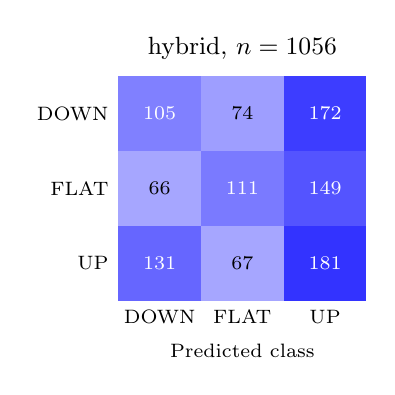
\begin{tikzpicture}[x=1.05cm,y=.95cm,font=\scriptsize]
\fill[blue!50] (0,2) rectangle ++(1,1);\node[text=white] at (0.5,2.5) {105};
\fill[blue!38] (1,2) rectangle ++(1,1);\node[text=black] at (1.5,2.5) {74};
\fill[blue!76] (2,2) rectangle ++(1,1);\node[text=white] at (2.5,2.5) {172};
\fill[blue!35] (0,1) rectangle ++(1,1);\node[text=black] at (0.5,1.5) {66};
\fill[blue!52] (1,1) rectangle ++(1,1);\node[text=white] at (1.5,1.5) {111};
\fill[blue!67] (2,1) rectangle ++(1,1);\node[text=white] at (2.5,1.5) {149};
\fill[blue!60] (0,0) rectangle ++(1,1);\node[text=white] at (0.5,0.5) {131};
\fill[blue!35] (1,0) rectangle ++(1,1);\node[text=black] at (1.5,0.5) {67};
\fill[blue!80] (2,0) rectangle ++(1,1);\node[text=white] at (2.5,0.5) {181};
\node[below] at (0.5,0) {DOWN};\node[left] at (0,2.5) {DOWN};
\node[below] at (1.5,0) {FLAT};\node[left] at (0,1.5) {FLAT};
\node[below] at (2.5,0) {UP};\node[left] at (0,0.5) {UP};
\node[above,font=\small] at (1.5,3.1) {hybrid, $n=1056$};
\node[below] at (1.5,-.45) {Predicted class};\end{tikzpicture}\end{minipage}
\hfill
\begin{minipage}[t]{.32\linewidth}\centering
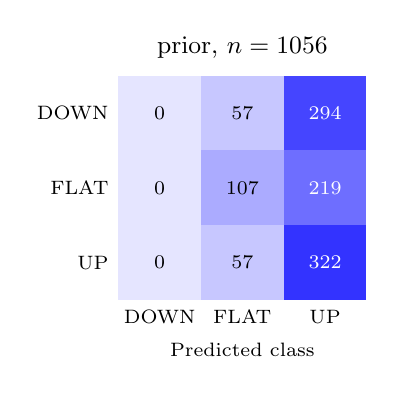
\begin{tikzpicture}[x=1.05cm,y=.95cm,font=\scriptsize]
\fill[blue!10] (0,2) rectangle ++(1,1);\node[text=black] at (0.5,2.5) {0};
\fill[blue!22] (1,2) rectangle ++(1,1);\node[text=black] at (1.5,2.5) {57};
\fill[blue!73] (2,2) rectangle ++(1,1);\node[text=white] at (2.5,2.5) {294};
\fill[blue!10] (0,1) rectangle ++(1,1);\node[text=black] at (0.5,1.5) {0};
\fill[blue!33] (1,1) rectangle ++(1,1);\node[text=black] at (1.5,1.5) {107};
\fill[blue!57] (2,1) rectangle ++(1,1);\node[text=white] at (2.5,1.5) {219};
\fill[blue!10] (0,0) rectangle ++(1,1);\node[text=black] at (0.5,0.5) {0};
\fill[blue!22] (1,0) rectangle ++(1,1);\node[text=black] at (1.5,0.5) {57};
\fill[blue!80] (2,0) rectangle ++(1,1);\node[text=white] at (2.5,0.5) {322};
\node[below] at (0.5,0) {DOWN};\node[left] at (0,2.5) {DOWN};
\node[below] at (1.5,0) {FLAT};\node[left] at (0,1.5) {FLAT};
\node[below] at (2.5,0) {UP};\node[left] at (0,0.5) {UP};
\node[above,font=\small] at (1.5,3.1) {prior, $n=1056$};
\node[below] at (1.5,-.45) {Predicted class};\end{tikzpicture}\end{minipage}
\hfill
\begin{minipage}[t]{.32\linewidth}\centering
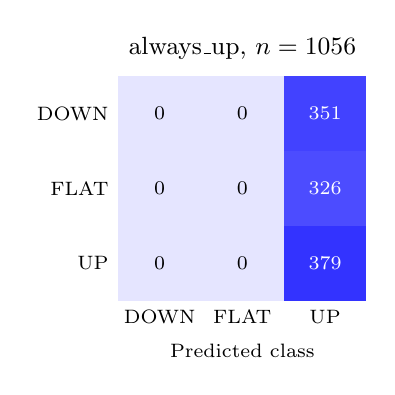
\begin{tikzpicture}[x=1.05cm,y=.95cm,font=\scriptsize]
\fill[blue!10] (0,2) rectangle ++(1,1);\node[text=black] at (0.5,2.5) {0};
\fill[blue!10] (1,2) rectangle ++(1,1);\node[text=black] at (1.5,2.5) {0};
\fill[blue!74] (2,2) rectangle ++(1,1);\node[text=white] at (2.5,2.5) {351};
\fill[blue!10] (0,1) rectangle ++(1,1);\node[text=black] at (0.5,1.5) {0};
\fill[blue!10] (1,1) rectangle ++(1,1);\node[text=black] at (1.5,1.5) {0};
\fill[blue!70] (2,1) rectangle ++(1,1);\node[text=white] at (2.5,1.5) {326};
\fill[blue!10] (0,0) rectangle ++(1,1);\node[text=black] at (0.5,0.5) {0};
\fill[blue!10] (1,0) rectangle ++(1,1);\node[text=black] at (1.5,0.5) {0};
\fill[blue!80] (2,0) rectangle ++(1,1);\node[text=white] at (2.5,0.5) {379};
\node[below] at (0.5,0) {DOWN};\node[left] at (0,2.5) {DOWN};
\node[below] at (1.5,0) {FLAT};\node[left] at (0,1.5) {FLAT};
\node[below] at (2.5,0) {UP};\node[left] at (0,0.5) {UP};
\node[above,font=\small] at (1.5,3.1) {always\_up, $n=1056$};
\node[below] at (1.5,-.45) {Predicted class};\end{tikzpicture}\end{minipage}
\caption{Audit confusion matrices with class support; row normalization does not create independent observations.}\label{fig:4}
\end{figure}

\noindent Table~\ref{tab:6} reports audit class report for calibrated mixture and prior.

\begin{table}[!htbp]\centering\footnotesize\setlength{\tabcolsep}{3pt}\renewcommand{\arraystretch}{1.14}
\caption{Audit class report for calibrated mixture and prior}\label{tab:6}
\begin{tabular}{@{}>{\raggedright\arraybackslash}p{\dimexpr 0.16667\textwidth-5.000pt\relax}>{\raggedright\arraybackslash}p{\dimexpr 0.16667\textwidth-5.000pt\relax}>{\raggedleft\arraybackslash}p{\dimexpr 0.16667\textwidth-5.000pt\relax}>{\raggedleft\arraybackslash}p{\dimexpr 0.16667\textwidth-5.000pt\relax}>{\raggedleft\arraybackslash}p{\dimexpr 0.16667\textwidth-5.000pt\relax}>{\raggedleft\arraybackslash}p{\dimexpr 0.16667\textwidth-5.000pt\relax}@{}}
\toprule
\textbf{Model} & \textbf{Class} & \textbf{Precision} & \textbf{Recall} & \textbf{F1} & \textbf{Support} \\
\midrule
hybrid & DOWN & 0.348 & 0.299 & 0.322 & 351 \\
hybrid & FLAT & 0.440 & 0.340 & 0.384 & 326 \\
hybrid & UP & 0.361 & 0.478 & 0.411 & 379 \\
prior & DOWN & 0.000 & 0.000 & 0.000 & 351 \\
prior & FLAT & 0.484 & 0.328 & 0.391 & 326 \\
prior & UP & 0.386 & 0.850 & 0.530 & 379 \\
\bottomrule\end{tabular}\par\smallskip
\raggedright\textit{Source:} \path{data/research-v2/tables/diag_class_report.csv}.
\end{table}


Per-class reporting prevents a common majority class from concealing weak recall elsewhere. Precision asks what fraction of a model's class assignments were right; recall asks how many observed examples of that class it recovered. F1 combines these two rates, and support states the denominator. Row-normalized confusion matrices emphasize which true classes are confused, while raw counts identify where most mistakes occur. The dominant transition can change when class prevalence changes even if the conditional error rates remain stable.

The most frequent off-diagonal transition in the audit is DOWN to UP, with 172 errors, or 49.00\% of that true class. Temperature scaling changes raw-mixture log loss by -0.0289 with interval [-0.0476, -0.0065]. The argmax labels are unchanged, as expected for positive temperature scaling. Better calibrated confidence can coexist with unchanged directional accuracy and still fail to beat the prior.

\noindent Figure~\ref{fig:5} shows probability reliability and confidence coverage, including bin support and uncertainty.

\begin{figure}[htbp]\centering
% Native editable figure; frozen statistics 0d291b4aebf8c524dc6705d872c070feb990e86a1cebbd59a758f400b240c952
\begin{minipage}[t]{.48\linewidth}\centering
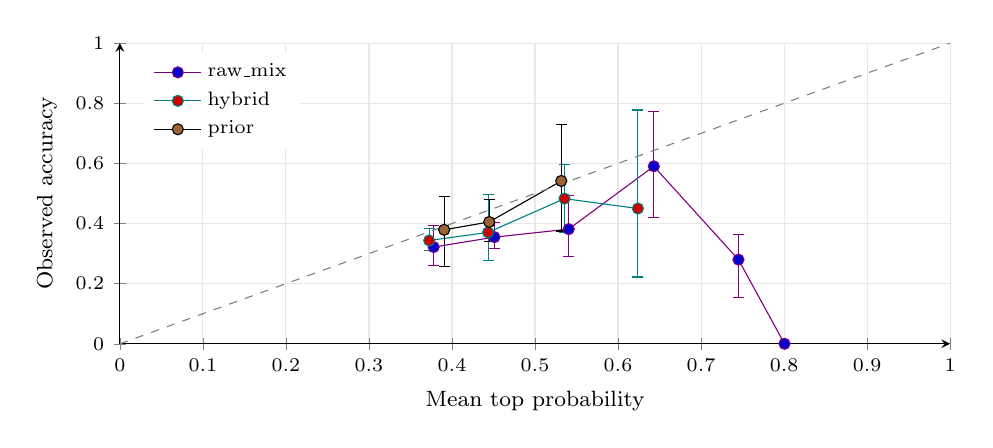
\begin{tikzpicture}
\begin{axis}[width=\linewidth,height=5.4cm,xmin=0,xmax=1,ymin=0,ymax=1,xlabel={Mean top probability},ylabel={Observed accuracy},legend pos=north west]
\addplot+[violet,mark=*,error bars/.cd,y dir=both,y explicit] table[x=x,y=y,y error minus=lo,y error plus=hi,row sep=\\]{x y lo hi\\0.377941396125 0.321739130435 0.061465157832 0.0711180124224\\
0.451112648618 0.354709418838 0.036937544687 0.0473755946032\\
0.540554545882 0.381381381381 0.0908637745748 0.112484584502\\
0.643079026906 0.590361445783 0.171317044239 0.182983792312\\
0.745038302803 0.28 0.12625 0.0836363636364\\
0.800526928081 0 0 0\\};
\addlegendentry{raw\_mix}
\addplot+[teal,mark=*,error bars/.cd,y dir=both,y explicit] table[x=x,y=y,y error minus=lo,y error plus=hi,row sep=\\]{x y lo hi\\0.372554098696 0.343680709534 0.033947623608 0.0388077697283\\
0.443490294143 0.370454545455 0.0928049251844 0.127299994627\\
0.535517133114 0.48275862069 0.113193403298 0.113135192247\\
0.62391873958 0.45 0.227777777778 0.327777777778\\};
\addlegendentry{hybrid}
\addplot+[black,mark=*,error bars/.cd,y dir=both,y explicit] table[x=x,y=y,y error minus=lo,y error plus=hi,row sep=\\]{x y lo hi\\0.390609751495 0.379146919431 0.123131687251 0.11015361194\\
0.444825090677 0.405269761606 0.0664880431194 0.0743930239297\\
0.531641069397 0.541666666667 0.166666666667 0.1875\\};
\addlegendentry{prior}
\addplot+[gray,mark=none,dashed] coordinates {(0,0) (1,1)};

\end{axis}
\end{tikzpicture}
\end{minipage}
\hfill
\begin{minipage}[t]{.48\linewidth}\centering
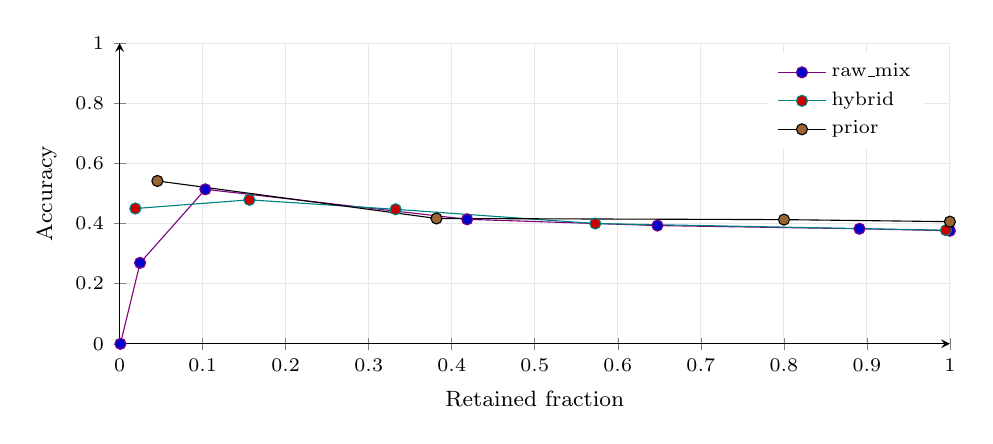
\begin{tikzpicture}
\begin{axis}[width=\linewidth,height=5.4cm,xmin=0,xmax=1,ymin=0,ymax=1,xlabel={Retained fraction},ylabel={Accuracy},legend pos=north east]
\addplot+[violet,mark=none,mark=*] coordinates {(1,0.375946969697) (0.891098484848,0.3825717322) (0.647727272727,0.393274853801) (0.418560606061,0.414027149321) (0.10321969697,0.51376146789) (0.0246212121212,0.269230769231) (0.00094696969697,0)};
\addlegendentry{raw\_mix}
\addplot+[teal,mark=none,mark=*] coordinates {(0.995265151515,0.37773549001) (0.572916666667,0.4) (0.332386363636,0.447293447293) (0.15625,0.478787878788) (0.0189393939394,0.45)};
\addlegendentry{hybrid}
\addplot+[black,mark=none,mark=*] coordinates {(1,0.40625) (0.800189393939,0.413017751479) (0.381628787879,0.416873449132) (0.0454545454545,0.541666666667)};
\addlegendentry{prior}

\end{axis}
\end{tikzpicture}
\end{minipage}
\caption{Probability reliability and confidence coverage, including bin support and uncertainty.}\label{fig:5}
\end{figure}

\noindent Table~\ref{tab:7} reports audit mixture confidence coverage; thresholds fixed for description.

\begin{table}[!htbp]\centering\footnotesize\setlength{\tabcolsep}{3pt}\renewcommand{\arraystretch}{1.14}
\caption{Audit mixture confidence coverage; thresholds fixed for description}\label{tab:7}
\begin{tabular}{@{}>{\raggedleft\arraybackslash}p{\dimexpr 0.20000\textwidth-4.800pt\relax}>{\raggedleft\arraybackslash}p{\dimexpr 0.20000\textwidth-4.800pt\relax}>{\raggedleft\arraybackslash}p{\dimexpr 0.20000\textwidth-4.800pt\relax}>{\raggedleft\arraybackslash}p{\dimexpr 0.20000\textwidth-4.800pt\relax}>{\raggedleft\arraybackslash}p{\dimexpr 0.20000\textwidth-4.800pt\relax}@{}}
\toprule
\textbf{Threshold} & \textbf{Retained} & \textbf{Dates} & \textbf{Coverage} & \textbf{Accuracy} \\
\midrule
0.34 & 1,051 & 48 & 99.53\% & 37.77\% \\
0.40 & 605 & 48 & 57.29\% & 40.00\% \\
0.45 & 351 & 48 & 33.24\% & 44.73\% \\
0.50 & 165 & 48 & 15.62\% & 47.88\% \\
0.60 & 20 & 15 & 1.89\% & 45.00\% \\
0.70 & 0 & 0 & 0.00\% & - \\
0.80 & 0 & 0 & 0.00\% & - \\
0.90 & 0 & 0 & 0.00\% & - \\
\bottomrule\end{tabular}\par\smallskip
\raggedright\textit{Source:} \path{data/research-v2/tables/diag_coverage.csv}.
\end{table}


Confidence-coverage curves retain only predictions above fixed confidence cutoffs and report both accuracy and remaining observations. A higher accuracy at low coverage can be practically irrelevant when almost no decisions remain. These curves are diagnostics, not an opportunity to choose the best threshold after viewing outcomes. Reliability-bin uncertainty is also limited by correlated dates; bins with little support cannot justify a confident calibration claim. For trading, an apparently well-calibrated probability still needs useful class-return estimates and enough expected advantage to pay costs.

\noindent Figure~\ref{fig:6} shows paired audit forecast effects and date-block uncertainty. Lower log loss is better.

\begin{figure}[htbp]\centering
% Native editable figure; frozen statistics 0d291b4aebf8c524dc6705d872c070feb990e86a1cebbd59a758f400b240c952
\begin{minipage}[t]{.32\linewidth}\centering
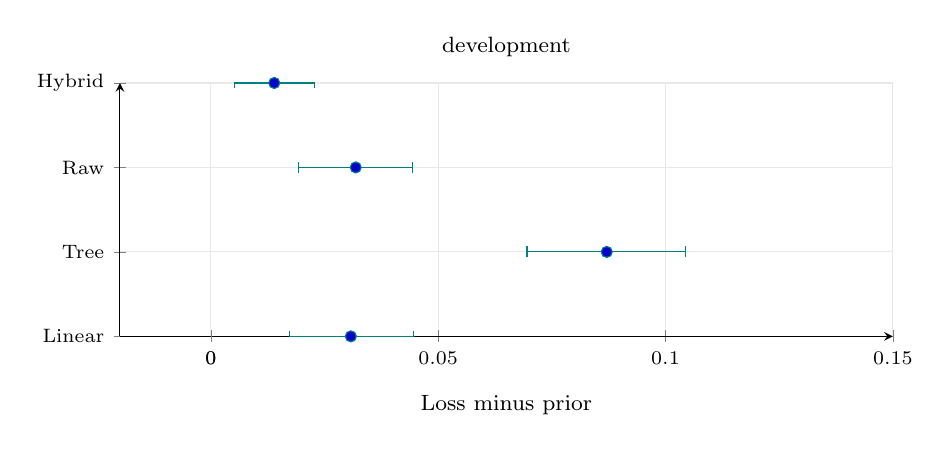
\begin{tikzpicture}
\begin{axis}[width=.94\linewidth,height=4.8cm,title={development},ytick={0,1,2,3},yticklabels={Linear,Tree,Raw,Hybrid},xlabel={Loss minus prior},xmin=-.02,xmax=.15,xtick={0,.05,.10,.15},scaled x ticks=false,x tick label style={/pgf/number format/fixed,/pgf/number format/precision=2},extra x ticks={0},extra x tick style={grid=major}]
\addplot+[teal,only marks,mark=*,error bars/.cd,x dir=both,x explicit] table[x=x,y=y,x error minus=lo,x error plus=hi,row sep=\\]{x y lo hi\\0.0307945818317 0 0.0133978723424 0.0138576511937\\
0.0870756476825 1 0.0175279184931 0.0174131845911\\
0.0318687091039 2 0.0126557943824 0.0125213618115\\
0.013947459402 3 0.00878659866028 0.00885623096892\\};

\end{axis}
\end{tikzpicture}
\end{minipage}
\hfill
\begin{minipage}[t]{.32\linewidth}\centering
\begin{tikzpicture}
\begin{axis}[width=.94\linewidth,height=4.8cm,title={selection},ytick={0,1,2,3},yticklabels={Linear,Tree,Raw,Hybrid},xlabel={Loss minus prior},xmin=-.02,xmax=.15,xtick={0,.05,.10,.15},scaled x ticks=false,x tick label style={/pgf/number format/fixed,/pgf/number format/precision=2},extra x ticks={0},extra x tick style={grid=major}]
\addplot+[teal,only marks,mark=*,error bars/.cd,x dir=both,x explicit] table[x=x,y=y,x error minus=lo,x error plus=hi,row sep=\\]{x y lo hi\\0.0366086965343 0 0.0255516950915 0.0246095487994\\
0.0812901260331 1 0.0371062104379 0.0344655441593\\
0.030095155111 2 0.0201815717422 0.0184559397131\\
0.0050018252014 3 0.0178401338044 0.0180481599458\\};

\end{axis}
\end{tikzpicture}
\end{minipage}
\hfill
\begin{minipage}[t]{.32\linewidth}\centering
\begin{tikzpicture}
\begin{axis}[width=.94\linewidth,height=4.8cm,title={audit},ytick={0,1,2,3},yticklabels={Linear,Tree,Raw,Hybrid},xlabel={Loss minus prior},xmin=-.02,xmax=.15,xtick={0,.05,.10,.15},scaled x ticks=false,x tick label style={/pgf/number format/fixed,/pgf/number format/precision=2},extra x ticks={0},extra x tick style={grid=major}]
\addplot+[teal,only marks,mark=*,error bars/.cd,x dir=both,x explicit] table[x=x,y=y,x error minus=lo,x error plus=hi,row sep=\\]{x y lo hi\\0.0534971109377 0 0.0225075059482 0.0232500211536\\
0.0923489707796 1 0.0408988275295 0.0429054660783\\
0.0415131268524 2 0.0186156550241 0.0193978388432\\
0.0126044345825 3 0.0150693518368 0.0143454615776\\};

\end{axis}
\end{tikzpicture}
\end{minipage}
\caption{Paired audit forecast effects and date-block uncertainty. Lower log loss is better.}\label{fig:6}
\end{figure}

For the primary audit hybrid-minus-prior comparison, the estimated loss difference is 0.0126, the bootstrap standard error is 0.0076, and the approximate 80\%-power detectable magnitude is 0.0213. With 48 dates and primary blocks of 10 dates, the effective information is much smaller than the number of stock rows suggests. This approximation ignores additional uncertainty about structural change and is not a prospective power guarantee.

\section{Controlled ablations, adaptation and transfer}\label{sec:section-07}

R5-momentum: candidate-minus-reference log loss -0.0022 (lower loss), 95\% interval [-0.0099, 0.0057], Holm p=1.000. R5-trend: candidate-minus-reference log loss 0.0027 (higher loss), 95\% interval [-0.0020, 0.0075], Holm p=1.000. R5-risk: candidate-minus-reference log loss -0.0021 (lower loss), 95\% interval [-0.0097, 0.0054], Holm p=1.000. R5-context\_volume: candidate-minus-reference log loss 0.0053 (higher loss), 95\% interval [0.0005, 0.0100], Holm p=0.243.

\noindent Table~\ref{tab:8} reports controlled feature ablations.

\begin{table}[!htbp]\centering\footnotesize\setlength{\tabcolsep}{3pt}\renewcommand{\arraystretch}{1.14}
\caption{Controlled feature ablations}\label{tab:8}
\begin{tabular}{@{}>{\raggedright\arraybackslash}p{\dimexpr 0.25758\textwidth-5.000pt\relax}>{\raggedleft\arraybackslash}p{\dimexpr 0.14773\textwidth-5.000pt\relax}>{\raggedleft\arraybackslash}p{\dimexpr 0.15152\textwidth-5.000pt\relax}>{\raggedleft\arraybackslash}p{\dimexpr 0.14773\textwidth-5.000pt\relax}>{\raggedleft\arraybackslash}p{\dimexpr 0.14773\textwidth-5.000pt\relax}>{\raggedleft\arraybackslash}p{\dimexpr 0.14773\textwidth-5.000pt\relax}@{}}
\toprule
\textbf{Contrast} & \textbf{Rows} & \textbf{Loss delta} & \textbf{CI low} & \textbf{CI high} & \textbf{Holm p} \\
\midrule
R5-momentum & 5,544 & -0.0022 & -0.0099 & 0.0057 & 1.000 \\
R5-trend & 5,544 & 0.0027 & -0.0020 & 0.0075 & 1.000 \\
R5-risk & 5,544 & -0.0021 & -0.0097 & 0.0054 & 1.000 \\
R5-context\_\allowbreak{}volume & 5,544 & 0.0053 & 0.0005 & 0.0100 & 0.243 \\
\bottomrule\end{tabular}\par\smallskip
\raggedright\textit{Source:} \path{data/research-v2/tables/exp_contrasts.csv}.
\end{table}


\noindent Figure~\ref{fig:7} shows registered controlled contrasts on development outer blocks; intervals preserve date dependence.

\begin{figure}[htbp]\centering
% Native editable figure; frozen statistics 0d291b4aebf8c524dc6705d872c070feb990e86a1cebbd59a758f400b240c952
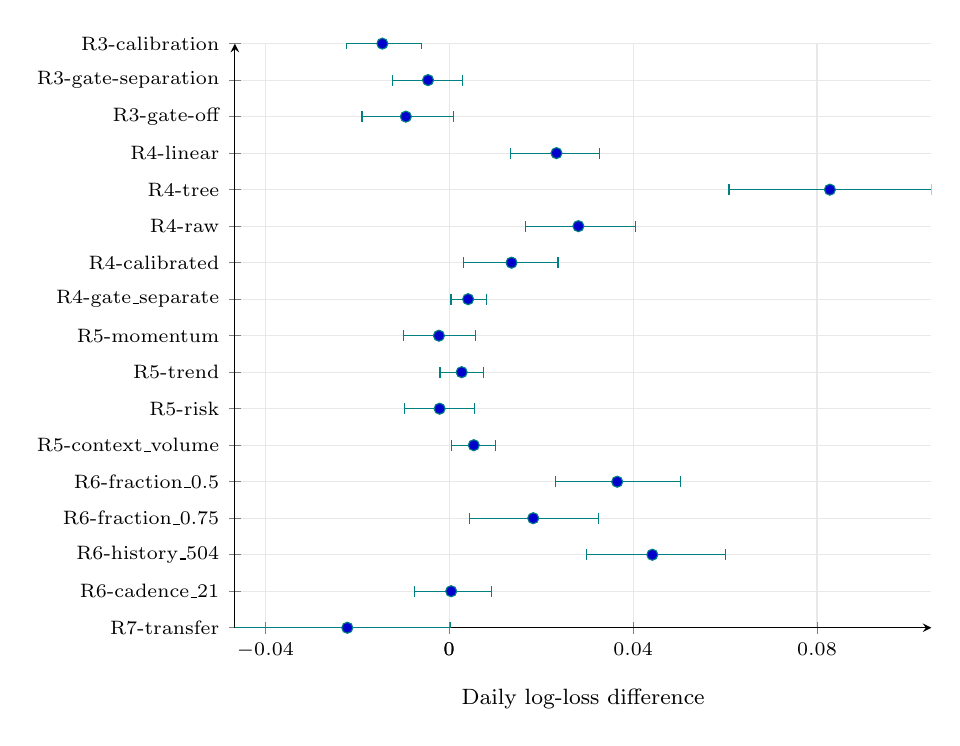
\begin{tikzpicture}
\begin{axis}[width=.86\linewidth,height=9cm,ytick={0,1,2,3,4,5,6,7,8,9,10,11,12,13,14,15,16},yticklabels={{R7-transfer},{R6-cadence\_21},{R6-history\_504},{R6-fraction\_0.75},{R6-fraction\_0.5},{R5-context\_volume},{R5-risk},{R5-trend},{R5-momentum},{R4-gate\_separate},{R4-calibrated},{R4-raw},{R4-tree},{R4-linear},{R3-gate-off},{R3-gate-separation},{R3-calibration}},xlabel={Daily log-loss difference},scaled x ticks=false,xtick={-.04,0,.04,.08,.12},x tick label style={/pgf/number format/fixed,/pgf/number format/precision=2},extra x ticks={0},extra x tick style={grid=major}]
\addplot+[teal,only marks,mark=*,error bars/.cd,x dir=both,x explicit] table[x=x,y=y,x error minus=lo,x error plus=hi,row sep=\\]{x y lo hi\\-0.0221801343161 0 0.024455579808 0.0223931852201\\
0.00041632232384 1 0.00791390874367 0.00868206037013\\
0.0441811010945 2 0.0143275954856 0.015861729419\\
0.0182631117218 3 0.0138705225454 0.0141196775605\\
0.0365366597573 4 0.0133799431661 0.0137957905223\\
0.00533639532695 5 0.00486071784276 0.00466252994581\\
-0.00209736606647 6 0.00755715195286 0.00749668667262\\
0.00269779404642 7 0.00471778582188 0.00481513474751\\
-0.00224943558219 8 0.00768731950008 0.00793827176469\\
0.00410115278394 9 0.00372147435029 0.00402768313738\\
0.0135461882894 10 0.0104981010291 0.0101189671534\\
0.028097358561 11 0.0115527059594 0.0123625312577\\
0.0828103310099 12 0.0219448112081 0.0220977857158\\
0.0233234605807 13 0.0100885775788 0.00930814049429\\
-0.00944503550542 14 0.00953611262778 0.0104141759139\\
-0.00461796099919 15 0.00779347490533 0.00755609905958\\
-0.0145511702716 16 0.00775600532129 0.00857025671815\\};

\end{axis}
\end{tikzpicture}

\caption{Registered controlled contrasts on development outer blocks; intervals preserve date dependence.}\label{fig:7}
\end{figure}

A feature-importance ranking is not a feature ablation. The experiments remove a registered feature family, refit the eligible model and compare outer predictions on matching dates. This evaluates the value of allowing that family under the stated model and budget. Correlated families can substitute for one another; removing one does not estimate an isolated economic causal effect. The sign of an ablation also depends on regularization and sampling variance. We retain unfavorable and near-zero changes alongside any improvement.

R3-calibration: candidate-minus-reference log loss -0.0146 (lower loss), 95\% interval [-0.0223, -0.0060], Holm p=0.018. R3-gate-separation: candidate-minus-reference log loss -0.0046 (lower loss), 95\% interval [-0.0124, 0.0029], Holm p=1.000. R3-gate-off: candidate-minus-reference log loss -0.0094 (lower loss), 95\% interval [-0.0190, 0.0010], Holm p=0.458. The forecast gate here chooses between calibrated predictions and the prior as a diagnostic view. The portfolio gate separately controls the trend/ML weight. Neither is silently substituted for the frozen trend shadow.

\noindent Table~\ref{tab:9} reports controlled base forecast views on development outer blocks.

\begin{table}[!htbp]\centering\footnotesize\setlength{\tabcolsep}{3pt}\renewcommand{\arraystretch}{1.14}
\caption{Controlled base forecast views on development outer blocks}\label{tab:9}
\begin{tabular}{@{}>{\raggedright\arraybackslash}p{\dimexpr 0.20000\textwidth-5.000pt\relax}>{\raggedleft\arraybackslash}p{\dimexpr 0.15000\textwidth-5.000pt\relax}>{\raggedleft\arraybackslash}p{\dimexpr 0.15000\textwidth-5.000pt\relax}>{\raggedleft\arraybackslash}p{\dimexpr 0.15000\textwidth-5.000pt\relax}>{\raggedleft\arraybackslash}p{\dimexpr 0.15000\textwidth-5.000pt\relax}>{\raggedleft\arraybackslash}p{\dimexpr 0.20000\textwidth-5.000pt\relax}@{}}
\toprule
\textbf{View} & \textbf{Rows} & \textbf{Accuracy} & \textbf{Log loss} & \textbf{Brier} & \textbf{Separate gate} \\
\midrule
calibrated & 5,544 & 40.13\% & 1.0773 & 0.6549 & 27.27\% \\
gate\_\allowbreak{}same & 5,544 & 42.14\% & 1.0725 & 0.6516 & 27.27\% \\
gate\_\allowbreak{}separate & 5,544 & 41.94\% & 1.0679 & 0.6482 & 27.27\% \\
linear & 5,544 & 39.30\% & 1.0871 & 0.6628 & 27.27\% \\
prior & 5,544 & 42.19\% & 1.0638 & 0.6453 & 27.27\% \\
raw & 5,544 & 40.13\% & 1.0919 & 0.6657 & 27.27\% \\
tree & 5,544 & 40.22\% & 1.1466 & 0.6971 & 27.27\% \\
\bottomrule\end{tabular}\par\smallskip
\raggedright\textit{Source:} \path{data/research-v2/tables/exp_predictive.csv}.
\end{table}


R6-fraction\_0.5: candidate-minus-reference log loss 0.0365 (higher loss), 95\% interval [0.0232, 0.0503], Holm p=0.008. R6-fraction\_0.75: candidate-minus-reference log loss 0.0183 (higher loss), 95\% interval [0.0044, 0.0324], Holm p=0.082. R6-history\_504: candidate-minus-reference log loss 0.0442 (higher loss), 95\% interval [0.0299, 0.0600], Holm p=0.008. R6-cadence\_21: candidate-minus-reference log loss 0.0004 (higher loss), 95\% interval [-0.0075, 0.0091], Holm p=1.000.

\noindent Table~\ref{tab:10} reports controlled history, fraction and cadence contrasts.

\begin{table}[!htbp]\centering\footnotesize\setlength{\tabcolsep}{3pt}\renewcommand{\arraystretch}{1.14}
\caption{Controlled history, fraction and cadence contrasts}\label{tab:10}
\begin{tabular}{@{}>{\raggedright\arraybackslash}p{\dimexpr 0.24615\textwidth-5.000pt\relax}>{\raggedleft\arraybackslash}p{\dimexpr 0.15000\textwidth-5.000pt\relax}>{\raggedleft\arraybackslash}p{\dimexpr 0.15385\textwidth-5.000pt\relax}>{\raggedleft\arraybackslash}p{\dimexpr 0.15000\textwidth-5.000pt\relax}>{\raggedleft\arraybackslash}p{\dimexpr 0.15000\textwidth-5.000pt\relax}>{\raggedleft\arraybackslash}p{\dimexpr 0.15000\textwidth-5.000pt\relax}@{}}
\toprule
\textbf{Contrast} & \textbf{Rows} & \textbf{Loss delta} & \textbf{CI low} & \textbf{CI high} & \textbf{Holm p} \\
\midrule
R6-fraction\_\allowbreak{}0.5 & 5,544 & 0.0365 & 0.0232 & 0.0503 & 0.008 \\
R6-fraction\_\allowbreak{}0.75 & 5,544 & 0.0183 & 0.0044 & 0.0324 & 0.082 \\
R6-history\_\allowbreak{}504 & 5,544 & 0.0442 & 0.0299 & 0.0600 & 0.008 \\
R6-cadence\_\allowbreak{}21 & 1,512 & 0.0004 & -0.0075 & 0.0091 & 1.000 \\
\bottomrule\end{tabular}\par\smallskip
\raggedright\textit{Source:} \path{data/research-v2/tables/exp_contrasts.csv}.
\end{table}


\noindent Figure~\ref{fig:8} shows fitting versus outer validation log loss under training-design changes.

\begin{figure}[htbp]\centering
% Native editable figure; frozen statistics 0d291b4aebf8c524dc6705d872c070feb990e86a1cebbd59a758f400b240c952
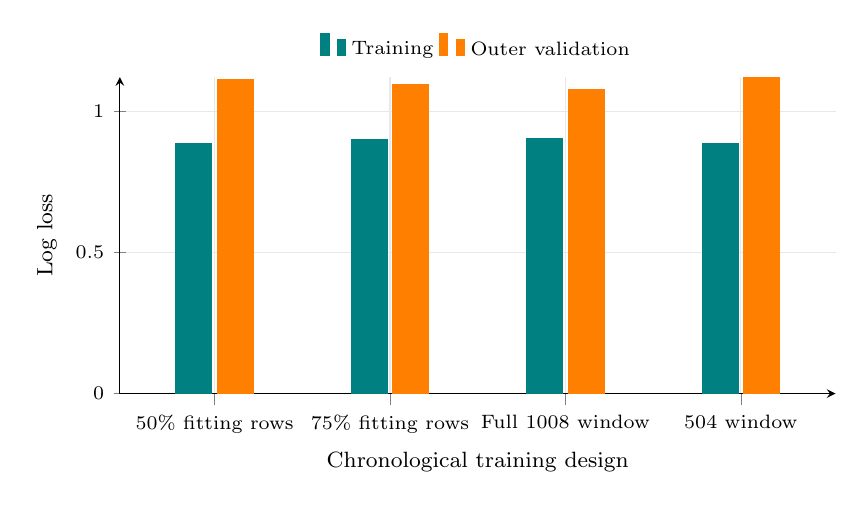
\begin{tikzpicture}
\begin{axis}[width=.88\linewidth,height=5.6cm,ybar,bar width=13pt,ymin=0,xtick={0,1,2,3},xticklabels={50\% fitting rows,75\% fitting rows,Full 1008 window,504 window},xlabel={Chronological training design},ylabel={Log loss},legend columns=2,legend style={at={(.5,1.02)},anchor=south},enlarge x limits=.18]
\addplot+[teal] coordinates {(0,0.885257437617) (1,0.899655741498) (2,0.904358782174) (3,0.887661478304)};
\addlegendentry{Training}
\addplot+[orange] coordinates {(0,1.11388215622) (1,1.09560860818) (2,1.07734549646) (3,1.12152659756)};
\addlegendentry{Outer validation}

\end{axis}
\end{tikzpicture}

\caption{Fitting versus outer validation log loss under training-design changes.}\label{fig:8}
\end{figure}

Across the registered seed comparisons, the largest probability difference is 0.0e+00. The tested deterministic estimator settings therefore produced identical probabilities across seeds. Zero seed variation is not zero research uncertainty: the calendar path, data vintage, history span and target instrument remain sources of variation. Shorter recent-history fractions change both row count and temporal span, so the learning curves do not identify a pure sample-size effect. Separating the gate also changes its recency as well as its information overlap.

Learning curves report fitting and outer-period loss together. A widening gap can be consistent with variance or time shift, while high loss on both partitions can indicate limited representation or model capacity. A smaller history can adapt faster but discard rare conditions; a larger history can stabilize estimation while retaining outdated relationships. Refit-cadence tests ask whether refreshing a fixed model matters under aligned information. No cadence is promoted merely because it is best on these consumed development blocks.

R7-transfer: candidate-minus-reference log loss -0.0222 (lower loss), 95\% interval [-0.0466, 0.0002], Holm p=0.458. The held-target comparison reports the aligned target subset only. Training on other instruments increases the number of fitting rows but does not increase the number of independent outer dates.

\noindent Table~\ref{tab:11} reports controlled held-instrument transfer contrast.

\begin{table}[!htbp]\centering\footnotesize\setlength{\tabcolsep}{3pt}\renewcommand{\arraystretch}{1.14}
\caption{Controlled held-instrument transfer contrast}\label{tab:11}
\begin{tabular}{@{}>{\raggedright\arraybackslash}p{\dimexpr 0.18333\textwidth-5.000pt\relax}>{\raggedleft\arraybackslash}p{\dimexpr 0.16250\textwidth-5.000pt\relax}>{\raggedleft\arraybackslash}p{\dimexpr 0.16667\textwidth-5.000pt\relax}>{\raggedleft\arraybackslash}p{\dimexpr 0.16250\textwidth-5.000pt\relax}>{\raggedleft\arraybackslash}p{\dimexpr 0.16250\textwidth-5.000pt\relax}>{\raggedleft\arraybackslash}p{\dimexpr 0.16250\textwidth-5.000pt\relax}@{}}
\toprule
\textbf{Contrast} & \textbf{Rows} & \textbf{Loss delta} & \textbf{CI low} & \textbf{CI high} & \textbf{Holm p} \\
\midrule
R7-transfer & 1,512 & -0.0222 & -0.0466 & 0.0002 & 0.458 \\
\bottomrule\end{tabular}\par\smallskip
\raggedright\textit{Source:} \path{data/research-v2/tables/exp_contrasts.csv}.
\end{table}


\noindent Figure~\ref{fig:9} shows historical instrument/period heterogeneity. Consumed-period slices are descriptive.

\begin{figure}[htbp]\centering
% Native editable figure; frozen statistics 0d291b4aebf8c524dc6705d872c070feb990e86a1cebbd59a758f400b240c952
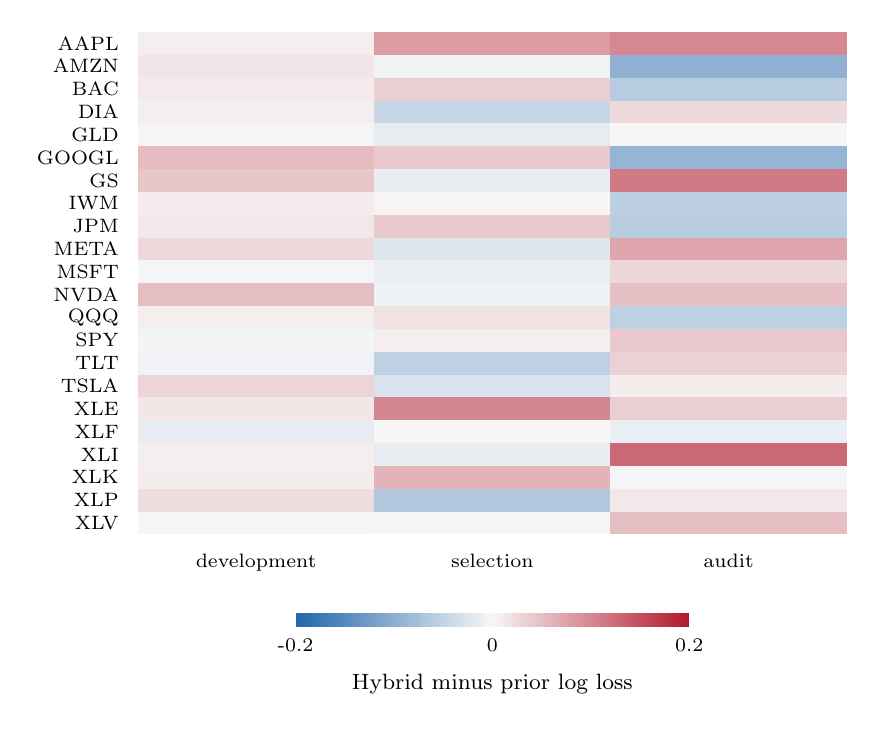
\begin{tikzpicture}[x=1cm,y=1cm,font=\scriptsize]
\node[anchor=east] at (-.12,6.235) {AAPL};
\fill[fill={rgb,255:red,244;green,238;blue,239}] (0,6.09) rectangle ++(3,0.29);
\fill[fill={rgb,255:red,219;green,156;blue,164}] (3,6.09) rectangle ++(3,0.29);
\fill[fill={rgb,255:red,213;green,136;blue,146}] (6,6.09) rectangle ++(3,0.29);
\node[anchor=east] at (-.12,5.945) {AMZN};
\fill[fill={rgb,255:red,241;green,229;blue,231}] (0,5.8) rectangle ++(3,0.29);
\fill[fill={rgb,255:red,242;green,243;blue,245}] (3,5.8) rectangle ++(3,0.29);
\fill[fill={rgb,255:red,144;green,177;blue,211}] (6,5.8) rectangle ++(3,0.29);
\node[anchor=east] at (-.12,5.655) {BAC};
\fill[fill={rgb,255:red,243;green,234;blue,235}] (0,5.51) rectangle ++(3,0.29);
\fill[fill={rgb,255:red,235;green,208;blue,211}] (3,5.51) rectangle ++(3,0.29);
\fill[fill={rgb,255:red,184;green,204;blue,225}] (6,5.51) rectangle ++(3,0.29);
\node[anchor=east] at (-.12,5.365) {DIA};
\fill[fill={rgb,255:red,244;green,238;blue,239}] (0,5.22) rectangle ++(3,0.29);
\fill[fill={rgb,255:red,198;green,214;blue,230}] (3,5.22) rectangle ++(3,0.29);
\fill[fill={rgb,255:red,238;green,218;blue,220}] (6,5.22) rectangle ++(3,0.29);
\node[anchor=east] at (-.12,5.075) {GLD};
\fill[fill={rgb,255:red,246;green,245;blue,245}] (0,4.93) rectangle ++(3,0.29);
\fill[fill={rgb,255:red,231;green,236;blue,241}] (3,4.93) rectangle ++(3,0.29);
\fill[fill={rgb,255:red,246;green,246;blue,246}] (6,4.93) rectangle ++(3,0.29);
\node[anchor=east] at (-.12,4.785) {GOOGL};
\fill[fill={rgb,255:red,229;green,188;blue,193}] (0,4.64) rectangle ++(3,0.29);
\fill[fill={rgb,255:red,233;green,201;blue,205}] (3,4.64) rectangle ++(3,0.29);
\fill[fill={rgb,255:red,150;green,181;blue,213}] (6,4.64) rectangle ++(3,0.29);
\node[anchor=east] at (-.12,4.495) {GS};
\fill[fill={rgb,255:red,232;green,199;blue,203}] (0,4.35) rectangle ++(3,0.29);
\fill[fill={rgb,255:red,233;green,237;blue,242}] (3,4.35) rectangle ++(3,0.29);
\fill[fill={rgb,255:red,208;green,122;blue,133}] (6,4.35) rectangle ++(3,0.29);
\node[anchor=east] at (-.12,4.205) {IWM};
\fill[fill={rgb,255:red,244;green,236;blue,237}] (0,4.06) rectangle ++(3,0.29);
\fill[fill={rgb,255:red,246;green,244;blue,244}] (3,4.06) rectangle ++(3,0.29);
\fill[fill={rgb,255:red,189;green,208;blue,227}] (6,4.06) rectangle ++(3,0.29);
\node[anchor=east] at (-.12,3.915) {JPM};
\fill[fill={rgb,255:red,242;green,232;blue,234}] (0,3.77) rectangle ++(3,0.29);
\fill[fill={rgb,255:red,233;green,201;blue,205}] (3,3.77) rectangle ++(3,0.29);
\fill[fill={rgb,255:red,185;green,205;blue,225}] (6,3.77) rectangle ++(3,0.29);
\node[anchor=east] at (-.12,3.625) {META};
\fill[fill={rgb,255:red,238;green,216;blue,219}] (0,3.48) rectangle ++(3,0.29);
\fill[fill={rgb,255:red,222;green,230;blue,238}] (3,3.48) rectangle ++(3,0.29);
\fill[fill={rgb,255:red,222;green,165;blue,172}] (6,3.48) rectangle ++(3,0.29);
\node[anchor=east] at (-.12,3.335) {MSFT};
\fill[fill={rgb,255:red,244;green,245;blue,246}] (0,3.19) rectangle ++(3,0.29);
\fill[fill={rgb,255:red,234;green,238;blue,242}] (3,3.19) rectangle ++(3,0.29);
\fill[fill={rgb,255:red,237;green,214;blue,217}] (6,3.19) rectangle ++(3,0.29);
\node[anchor=east] at (-.12,3.045) {NVDA};
\fill[fill={rgb,255:red,229;green,190;blue,195}] (0,2.9) rectangle ++(3,0.29);
\fill[fill={rgb,255:red,239;green,242;blue,244}] (3,2.9) rectangle ++(3,0.29);
\fill[fill={rgb,255:red,230;green,192;blue,196}] (6,2.9) rectangle ++(3,0.29);
\node[anchor=east] at (-.12,2.755) {QQQ};
\fill[fill={rgb,255:red,244;green,238;blue,239}] (0,2.61) rectangle ++(3,0.29);
\fill[fill={rgb,255:red,240;green,225;blue,226}] (3,2.61) rectangle ++(3,0.29);
\fill[fill={rgb,255:red,190;green,209;blue,227}] (6,2.61) rectangle ++(3,0.29);
\node[anchor=east] at (-.12,2.465) {SPY};
\fill[fill={rgb,255:red,242;green,244;blue,245}] (0,2.32) rectangle ++(3,0.29);
\fill[fill={rgb,255:red,244;green,238;blue,239}] (3,2.32) rectangle ++(3,0.29);
\fill[fill={rgb,255:red,232;green,200;blue,204}] (6,2.32) rectangle ++(3,0.29);
\node[anchor=east] at (-.12,2.175) {TLT};
\fill[fill={rgb,255:red,240;green,242;blue,245}] (0,2.03) rectangle ++(3,0.29);
\fill[fill={rgb,255:red,190;green,209;blue,227}] (3,2.03) rectangle ++(3,0.29);
\fill[fill={rgb,255:red,235;green,208;blue,212}] (6,2.03) rectangle ++(3,0.29);
\node[anchor=east] at (-.12,1.885) {TSLA};
\fill[fill={rgb,255:red,236;green,212;blue,215}] (0,1.74) rectangle ++(3,0.29);
\fill[fill={rgb,255:red,218;green,227;blue,237}] (3,1.74) rectangle ++(3,0.29);
\fill[fill={rgb,255:red,244;green,236;blue,237}] (6,1.74) rectangle ++(3,0.29);
\node[anchor=east] at (-.12,1.595) {XLE};
\fill[fill={rgb,255:red,242;green,230;blue,231}] (0,1.45) rectangle ++(3,0.29);
\fill[fill={rgb,255:red,212;green,134;blue,144}] (3,1.45) rectangle ++(3,0.29);
\fill[fill={rgb,255:red,234;green,206;blue,209}] (6,1.45) rectangle ++(3,0.29);
\node[anchor=east] at (-.12,1.305) {XLF};
\fill[fill={rgb,255:red,231;green,236;blue,241}] (0,1.16) rectangle ++(3,0.29);
\fill[fill={rgb,255:red,247;green,246;blue,246}] (3,1.16) rectangle ++(3,0.29);
\fill[fill={rgb,255:red,233;green,238;blue,242}] (6,1.16) rectangle ++(3,0.29);
\node[anchor=east] at (-.12,1.015) {XLI};
\fill[fill={rgb,255:red,244;green,238;blue,239}] (0,0.87) rectangle ++(3,0.29);
\fill[fill={rgb,255:red,232;green,237;blue,242}] (3,0.87) rectangle ++(3,0.29);
\fill[fill={rgb,255:red,203;green,104;blue,117}] (6,0.87) rectangle ++(3,0.29);
\node[anchor=east] at (-.12,0.725) {XLK};
\fill[fill={rgb,255:red,244;green,236;blue,237}] (0,0.58) rectangle ++(3,0.29);
\fill[fill={rgb,255:red,226;green,180;blue,186}] (3,0.58) rectangle ++(3,0.29);
\fill[fill={rgb,255:red,243;green,245;blue,246}] (6,0.58) rectangle ++(3,0.29);
\node[anchor=east] at (-.12,0.435) {XLP};
\fill[fill={rgb,255:red,239;green,220;blue,223}] (0,0.29) rectangle ++(3,0.29);
\fill[fill={rgb,255:red,177;green,200;blue,223}] (3,0.29) rectangle ++(3,0.29);
\fill[fill={rgb,255:red,242;green,231;blue,233}] (6,0.29) rectangle ++(3,0.29);
\node[anchor=east] at (-.12,0.145) {XLV};
\fill[fill={rgb,255:red,243;green,245;blue,246}] (0,0) rectangle ++(3,0.29);
\fill[fill={rgb,255:red,246;green,246;blue,246}] (3,0) rectangle ++(3,0.29);
\fill[fill={rgb,255:red,230;green,191;blue,196}] (6,0) rectangle ++(3,0.29);
\node[anchor=north,align=center] at (1.5,-.12) {development};
\node[anchor=north,align=center] at (4.5,-.12) {selection};
\node[anchor=north,align=center] at (7.5,-.12) {audit};
\fill[fill={rgb,255:red,35;green,103;blue,173}] (2,-1.18) rectangle ++(.051,.18);
\fill[fill={rgb,255:red,39;green,106;blue,174}] (2.05,-1.18) rectangle ++(.051,.18);
\fill[fill={rgb,255:red,44;green,109;blue,176}] (2.1,-1.18) rectangle ++(.051,.18);
\fill[fill={rgb,255:red,48;green,112;blue,177}] (2.15,-1.18) rectangle ++(.051,.18);
\fill[fill={rgb,255:red,52;green,115;blue,179}] (2.2,-1.18) rectangle ++(.051,.18);
\fill[fill={rgb,255:red,57;green,118;blue,180}] (2.25,-1.18) rectangle ++(.051,.18);
\fill[fill={rgb,255:red,61;green,121;blue,182}] (2.3,-1.18) rectangle ++(.051,.18);
\fill[fill={rgb,255:red,65;green,124;blue,183}] (2.35,-1.18) rectangle ++(.051,.18);
\fill[fill={rgb,255:red,69;green,127;blue,185}] (2.4,-1.18) rectangle ++(.051,.18);
\fill[fill={rgb,255:red,74;green,130;blue,186}] (2.45,-1.18) rectangle ++(.051,.18);
\fill[fill={rgb,255:red,78;green,132;blue,188}] (2.5,-1.18) rectangle ++(.051,.18);
\fill[fill={rgb,255:red,82;green,135;blue,189}] (2.55,-1.18) rectangle ++(.051,.18);
\fill[fill={rgb,255:red,86;green,138;blue,191}] (2.6,-1.18) rectangle ++(.051,.18);
\fill[fill={rgb,255:red,91;green,141;blue,192}] (2.65,-1.18) rectangle ++(.051,.18);
\fill[fill={rgb,255:red,95;green,144;blue,194}] (2.7,-1.18) rectangle ++(.051,.18);
\fill[fill={rgb,255:red,99;green,147;blue,195}] (2.75,-1.18) rectangle ++(.051,.18);
\fill[fill={rgb,255:red,104;green,150;blue,197}] (2.8,-1.18) rectangle ++(.051,.18);
\fill[fill={rgb,255:red,108;green,153;blue,198}] (2.85,-1.18) rectangle ++(.051,.18);
\fill[fill={rgb,255:red,112;green,156;blue,200}] (2.9,-1.18) rectangle ++(.051,.18);
\fill[fill={rgb,255:red,116;green,159;blue,201}] (2.95,-1.18) rectangle ++(.051,.18);
\fill[fill={rgb,255:red,121;green,161;blue,203}] (3,-1.18) rectangle ++(.051,.18);
\fill[fill={rgb,255:red,125;green,164;blue,204}] (3.05,-1.18) rectangle ++(.051,.18);
\fill[fill={rgb,255:red,129;green,167;blue,206}] (3.1,-1.18) rectangle ++(.051,.18);
\fill[fill={rgb,255:red,134;green,170;blue,207}] (3.15,-1.18) rectangle ++(.051,.18);
\fill[fill={rgb,255:red,138;green,173;blue,209}] (3.2,-1.18) rectangle ++(.051,.18);
\fill[fill={rgb,255:red,142;green,176;blue,210}] (3.25,-1.18) rectangle ++(.051,.18);
\fill[fill={rgb,255:red,146;green,179;blue,212}] (3.3,-1.18) rectangle ++(.051,.18);
\fill[fill={rgb,255:red,151;green,182;blue,213}] (3.35,-1.18) rectangle ++(.051,.18);
\fill[fill={rgb,255:red,155;green,185;blue,215}] (3.4,-1.18) rectangle ++(.051,.18);
\fill[fill={rgb,255:red,159;green,188;blue,216}] (3.45,-1.18) rectangle ++(.051,.18);
\fill[fill={rgb,255:red,164;green,190;blue,218}] (3.5,-1.18) rectangle ++(.051,.18);
\fill[fill={rgb,255:red,168;green,193;blue,219}] (3.55,-1.18) rectangle ++(.051,.18);
\fill[fill={rgb,255:red,172;green,196;blue,221}] (3.6,-1.18) rectangle ++(.051,.18);
\fill[fill={rgb,255:red,176;green,199;blue,222}] (3.65,-1.18) rectangle ++(.051,.18);
\fill[fill={rgb,255:red,181;green,202;blue,224}] (3.7,-1.18) rectangle ++(.051,.18);
\fill[fill={rgb,255:red,185;green,205;blue,225}] (3.75,-1.18) rectangle ++(.051,.18);
\fill[fill={rgb,255:red,189;green,208;blue,227}] (3.8,-1.18) rectangle ++(.051,.18);
\fill[fill={rgb,255:red,193;green,211;blue,228}] (3.85,-1.18) rectangle ++(.051,.18);
\fill[fill={rgb,255:red,198;green,214;blue,230}] (3.9,-1.18) rectangle ++(.051,.18);
\fill[fill={rgb,255:red,202;green,217;blue,231}] (3.95,-1.18) rectangle ++(.051,.18);
\fill[fill={rgb,255:red,206;green,219;blue,233}] (4,-1.18) rectangle ++(.051,.18);
\fill[fill={rgb,255:red,211;green,222;blue,234}] (4.05,-1.18) rectangle ++(.051,.18);
\fill[fill={rgb,255:red,215;green,225;blue,236}] (4.1,-1.18) rectangle ++(.051,.18);
\fill[fill={rgb,255:red,219;green,228;blue,237}] (4.15,-1.18) rectangle ++(.051,.18);
\fill[fill={rgb,255:red,223;green,231;blue,239}] (4.2,-1.18) rectangle ++(.051,.18);
\fill[fill={rgb,255:red,228;green,234;blue,240}] (4.25,-1.18) rectangle ++(.051,.18);
\fill[fill={rgb,255:red,232;green,237;blue,242}] (4.3,-1.18) rectangle ++(.051,.18);
\fill[fill={rgb,255:red,236;green,240;blue,243}] (4.35,-1.18) rectangle ++(.051,.18);
\fill[fill={rgb,255:red,241;green,243;blue,245}] (4.4,-1.18) rectangle ++(.051,.18);
\fill[fill={rgb,255:red,245;green,246;blue,246}] (4.45,-1.18) rectangle ++(.051,.18);
\fill[fill={rgb,255:red,246;green,245;blue,245}] (4.5,-1.18) rectangle ++(.051,.18);
\fill[fill={rgb,255:red,245;green,240;blue,241}] (4.55,-1.18) rectangle ++(.051,.18);
\fill[fill={rgb,255:red,244;green,236;blue,237}] (4.6,-1.18) rectangle ++(.051,.18);
\fill[fill={rgb,255:red,242;green,231;blue,233}] (4.65,-1.18) rectangle ++(.051,.18);
\fill[fill={rgb,255:red,241;green,227;blue,229}] (4.7,-1.18) rectangle ++(.051,.18);
\fill[fill={rgb,255:red,239;green,222;blue,225}] (4.75,-1.18) rectangle ++(.051,.18);
\fill[fill={rgb,255:red,238;green,218;blue,220}] (4.8,-1.18) rectangle ++(.051,.18);
\fill[fill={rgb,255:red,237;green,214;blue,216}] (4.85,-1.18) rectangle ++(.051,.18);
\fill[fill={rgb,255:red,235;green,209;blue,212}] (4.9,-1.18) rectangle ++(.051,.18);
\fill[fill={rgb,255:red,234;green,205;blue,208}] (4.95,-1.18) rectangle ++(.051,.18);
\fill[fill={rgb,255:red,233;green,200;blue,204}] (5,-1.18) rectangle ++(.051,.18);
\fill[fill={rgb,255:red,231;green,196;blue,200}] (5.05,-1.18) rectangle ++(.051,.18);
\fill[fill={rgb,255:red,230;green,191;blue,196}] (5.1,-1.18) rectangle ++(.051,.18);
\fill[fill={rgb,255:red,228;green,187;blue,192}] (5.15,-1.18) rectangle ++(.051,.18);
\fill[fill={rgb,255:red,227;green,182;blue,188}] (5.2,-1.18) rectangle ++(.051,.18);
\fill[fill={rgb,255:red,226;green,178;blue,184}] (5.25,-1.18) rectangle ++(.051,.18);
\fill[fill={rgb,255:red,224;green,173;blue,180}] (5.3,-1.18) rectangle ++(.051,.18);
\fill[fill={rgb,255:red,223;green,169;blue,176}] (5.35,-1.18) rectangle ++(.051,.18);
\fill[fill={rgb,255:red,221;green,164;blue,172}] (5.4,-1.18) rectangle ++(.051,.18);
\fill[fill={rgb,255:red,220;green,160;blue,167}] (5.45,-1.18) rectangle ++(.051,.18);
\fill[fill={rgb,255:red,219;green,156;blue,163}] (5.5,-1.18) rectangle ++(.051,.18);
\fill[fill={rgb,255:red,217;green,151;blue,159}] (5.55,-1.18) rectangle ++(.051,.18);
\fill[fill={rgb,255:red,216;green,147;blue,155}] (5.6,-1.18) rectangle ++(.051,.18);
\fill[fill={rgb,255:red,215;green,142;blue,151}] (5.65,-1.18) rectangle ++(.051,.18);
\fill[fill={rgb,255:red,213;green,138;blue,147}] (5.7,-1.18) rectangle ++(.051,.18);
\fill[fill={rgb,255:red,212;green,133;blue,143}] (5.75,-1.18) rectangle ++(.051,.18);
\fill[fill={rgb,255:red,210;green,129;blue,139}] (5.8,-1.18) rectangle ++(.051,.18);
\fill[fill={rgb,255:red,209;green,124;blue,135}] (5.85,-1.18) rectangle ++(.051,.18);
\fill[fill={rgb,255:red,208;green,120;blue,131}] (5.9,-1.18) rectangle ++(.051,.18);
\fill[fill={rgb,255:red,206;green,115;blue,127}] (5.95,-1.18) rectangle ++(.051,.18);
\fill[fill={rgb,255:red,205;green,111;blue,123}] (6,-1.18) rectangle ++(.051,.18);
\fill[fill={rgb,255:red,204;green,107;blue,118}] (6.05,-1.18) rectangle ++(.051,.18);
\fill[fill={rgb,255:red,202;green,102;blue,114}] (6.1,-1.18) rectangle ++(.051,.18);
\fill[fill={rgb,255:red,201;green,98;blue,110}] (6.15,-1.18) rectangle ++(.051,.18);
\fill[fill={rgb,255:red,199;green,93;blue,106}] (6.2,-1.18) rectangle ++(.051,.18);
\fill[fill={rgb,255:red,198;green,89;blue,102}] (6.25,-1.18) rectangle ++(.051,.18);
\fill[fill={rgb,255:red,197;green,84;blue,98}] (6.3,-1.18) rectangle ++(.051,.18);
\fill[fill={rgb,255:red,195;green,80;blue,94}] (6.35,-1.18) rectangle ++(.051,.18);
\fill[fill={rgb,255:red,194;green,75;blue,90}] (6.4,-1.18) rectangle ++(.051,.18);
\fill[fill={rgb,255:red,192;green,71;blue,86}] (6.45,-1.18) rectangle ++(.051,.18);
\fill[fill={rgb,255:red,191;green,66;blue,82}] (6.5,-1.18) rectangle ++(.051,.18);
\fill[fill={rgb,255:red,190;green,62;blue,78}] (6.55,-1.18) rectangle ++(.051,.18);
\fill[fill={rgb,255:red,188;green,57;blue,74}] (6.6,-1.18) rectangle ++(.051,.18);
\fill[fill={rgb,255:red,187;green,53;blue,70}] (6.65,-1.18) rectangle ++(.051,.18);
\fill[fill={rgb,255:red,186;green,49;blue,65}] (6.7,-1.18) rectangle ++(.051,.18);
\fill[fill={rgb,255:red,184;green,44;blue,61}] (6.75,-1.18) rectangle ++(.051,.18);
\fill[fill={rgb,255:red,183;green,40;blue,57}] (6.8,-1.18) rectangle ++(.051,.18);
\fill[fill={rgb,255:red,181;green,35;blue,53}] (6.85,-1.18) rectangle ++(.051,.18);
\fill[fill={rgb,255:red,180;green,31;blue,49}] (6.9,-1.18) rectangle ++(.051,.18);
\fill[fill={rgb,255:red,179;green,26;blue,45}] (6.95,-1.18) rectangle ++(.051,.18);
\node[anchor=north] at (2,-1.2) {-0.2};
\node[anchor=north] at (4.5,-1.2) {0};
\node[anchor=north] at (7,-1.2) {0.2};
\node[anchor=north,font=\footnotesize] at (4.5,-1.65) {Hybrid minus prior log loss};
\end{tikzpicture}
\caption{Historical instrument/period heterogeneity. Consumed-period slices are descriptive.}\label{fig:9}
\end{figure}

The instrument-transfer experiment withholds target instruments from pooled fitting and respects the temporal outer boundary. That is stronger than reporting each single-instrument model on its own later observations, but it is still limited by overlapping economic exposures and a shared market feature. Excluding an instrument's labels does not remove all information about the market in which it trades. Transfer results therefore describe the declared source/target grouping, not universal generalization to unseen exchanges or delisted securities.

Regime slices use conditions observable at the decision time. Realized future volatility is not used to assign a model's historical input state. Support counts accompany every slice, because a dramatic result from few dates is less stable than an aggregate over many market episodes. Instrument, period and regime analyses describe heterogeneity; they do not license a selector trained retrospectively to keep only the favorable cells.

\section{Economic performance, costs and failure mechanisms}\label{sec:section-08}

The controlled portfolio comparisons do not establish an economic advantage: every primary-block interval below crosses zero after matching the same outer dates and execution rules. Each fold starts a fresh account; the study averages daily active returns across those blocks, not a fictitious continuously invested equity path across the intervening gaps. Approximate detectable daily active effects range from 0.0420\% to 0.0736\%. These are large relative to the registered practical threshold. The bootstrap conditions on the observed outer blocks and cannot establish robustness to an unseen market regime.

\noindent Table~\ref{tab:12} reports controlled daily active returns versus equal weight; primary date-block inference.

\begin{table}[!htbp]\centering\footnotesize\setlength{\tabcolsep}{3pt}\renewcommand{\arraystretch}{1.14}
\caption{Controlled daily active returns versus equal weight; primary date-block inference}\label{tab:12}
\begin{tabular}{@{}>{\raggedright\arraybackslash}p{\dimexpr 0.20312\textwidth-5.000pt\relax}>{\raggedleft\arraybackslash}p{\dimexpr 0.15234\textwidth-5.000pt\relax}>{\raggedleft\arraybackslash}p{\dimexpr 0.18750\textwidth-5.000pt\relax}>{\raggedleft\arraybackslash}p{\dimexpr 0.15234\textwidth-5.000pt\relax}>{\raggedleft\arraybackslash}p{\dimexpr 0.15234\textwidth-5.000pt\relax}>{\raggedleft\arraybackslash}p{\dimexpr 0.15234\textwidth-5.000pt\relax}@{}}
\toprule
\textbf{Policy} & \textbf{Dates} & \textbf{Daily effect} & \textbf{CI low} & \textbf{CI high} & \textbf{Holm p} \\
\midrule
linear & 252 & -0.04\% & -0.08\% & 0.01\% & 0.972 \\
tree & 252 & -0.00\% & -0.05\% & 0.04\% & 1.000 \\
raw & 252 & -0.02\% & -0.06\% & 0.02\% & 1.000 \\
calibrated & 252 & -0.03\% & -0.08\% & 0.02\% & 1.000 \\
fixed\_\allowbreak{}mix & 252 & -0.01\% & -0.05\% & 0.02\% & 1.000 \\
same\_\allowbreak{}gate & 252 & -0.01\% & -0.04\% & 0.02\% & 1.000 \\
separate\_\allowbreak{}gate & 252 & -0.00\% & -0.03\% & 0.03\% & 1.000 \\
trend & 252 & -0.00\% & -0.03\% & 0.03\% & 1.000 \\
\bottomrule\end{tabular}\par\smallskip
\raggedright\textit{Source:} \path{data/research-v2/tables/exp_economic_contrasts.csv}.
\end{table}


For the newly matched audit accounts, each policy begins with 10,000.00 dollars. The adaptive hybrid ends at 9,954.29 dollars and the equal-weight control at 10,254.73 dollars. Hybrid net return is -0.46\%, maximum drawdown -2.21\%, and average gross exposure 55.63\%. These fresh-capital results differ from the sealed continuous-account audit because startup holdings and entry financing differ. The continuous curves below retain their original account history and are labeled accordingly.

\noindent Table~\ref{tab:13} reports fresh-capital audit accounts; zero-rate Sharpe and modeled per-side costs.

\begin{table}[!htbp]\centering\footnotesize\setlength{\tabcolsep}{3pt}\renewcommand{\arraystretch}{1.14}
\caption{Fresh-capital audit accounts; zero-rate Sharpe and modeled per-side costs}\label{tab:13}
\begin{tabular}{@{}>{\raggedright\arraybackslash}p{\dimexpr 0.20339\textwidth-5.143pt\relax}>{\raggedleft\arraybackslash}p{\dimexpr 0.13559\textwidth-5.143pt\relax}>{\raggedleft\arraybackslash}p{\dimexpr 0.13220\textwidth-5.143pt\relax}>{\raggedleft\arraybackslash}p{\dimexpr 0.13220\textwidth-5.143pt\relax}>{\raggedleft\arraybackslash}p{\dimexpr 0.13220\textwidth-5.143pt\relax}>{\raggedleft\arraybackslash}p{\dimexpr 0.13220\textwidth-5.143pt\relax}>{\raggedleft\arraybackslash}p{\dimexpr 0.13220\textwidth-5.143pt\relax}@{}}
\toprule
\textbf{Policy} & \textbf{Net return} & \textbf{Sharpe} & \textbf{Max DD} & \textbf{Exposure} & \textbf{Costs (\$)} & \textbf{Fills} \\
\midrule
trend & -0.48\% & -0.328 & -2.34\% & 56.67\% & 15.24 & 184 \\
ml & -0.48\% & -0.360 & -2.13\% & 32.22\% & 29.57 & 119 \\
adaptive\_\allowbreak{}hybrid & -0.46\% & -0.309 & -2.21\% & 55.63\% & 20.51 & 217 \\
equal\_\allowbreak{}weight & 2.55\% & 1.297 & -2.66\% & 74.45\% & 13.58 & 205 \\
cash & 0.00\% & - & 0.00\% & 0.00\% & 0.00 & 0 \\
\bottomrule\end{tabular}\par\smallskip
\raggedright\textit{Source:} \path{data/research-v2/tables/diag_portfolio.csv}.
\end{table}


\noindent Figure~\ref{fig:10} shows continuous accounts from their original common start; these are not fresh audit allocations.

\begin{figure}[htbp]\centering
% Native editable figure; frozen statistics 0d291b4aebf8c524dc6705d872c070feb990e86a1cebbd59a758f400b240c952
\begin{tikzpicture}\begin{groupplot}[group style={group size=1 by 3,vertical sep=9mm},width=.90\linewidth,height=4.1cm,scaled y ticks=false,y tick label style={/pgf/number format/fixed,/pgf/number format/precision=2},xmin=0,xmax=685,xtick={0,125,251,376,502,625,685},xticklabels={Jan24,Jul24,Jan25,Jul25,Jan26,Jul26,Sep26}]
\nextgroupplot[ylabel={Equity (USD)},legend columns=3,legend style={at={(.5,1.06)},anchor=south},xticklabels=\empty]
\addplot+[blue,mark=none,thin] table[col sep=comma,x=session_index,y=equity] {data/portfolio-trend.csv};
\addlegendentry{trend}
\addplot+[orange,mark=none,thin] table[col sep=comma,x=session_index,y=equity] {data/portfolio-ml.csv};
\addlegendentry{ml}
\addplot+[teal,mark=none,thin] table[col sep=comma,x=session_index,y=equity] {data/portfolio-adaptive_hybrid.csv};
\addlegendentry{adaptive\_hybrid}
\addplot+[black,mark=none,thin] table[col sep=comma,x=session_index,y=equity] {data/portfolio-equal_weight.csv};
\addlegendentry{equal\_weight}
\addplot+[gray,mark=none,thin] table[col sep=comma,x=session_index,y=equity] {data/portfolio-cash.csv};
\addlegendentry{cash}
\nextgroupplot[ylabel={Drawdown (fraction)},xticklabels=\empty]
\addplot+[blue,mark=none,thin] table[col sep=comma,x=session_index,y=drawdown] {data/portfolio-trend.csv};
\addplot+[orange,mark=none,thin] table[col sep=comma,x=session_index,y=drawdown] {data/portfolio-ml.csv};
\addplot+[teal,mark=none,thin] table[col sep=comma,x=session_index,y=drawdown] {data/portfolio-adaptive_hybrid.csv};
\addplot+[black,mark=none,thin] table[col sep=comma,x=session_index,y=drawdown] {data/portfolio-equal_weight.csv};
\addplot+[gray,mark=none,thin] table[col sep=comma,x=session_index,y=drawdown] {data/portfolio-cash.csv};
\nextgroupplot[ylabel={Gross exposure}]
\addplot+[blue,mark=none,thin] table[col sep=comma,x=session_index,y=exposure] {data/portfolio-trend.csv};
\addplot+[orange,mark=none,thin] table[col sep=comma,x=session_index,y=exposure] {data/portfolio-ml.csv};
\addplot+[teal,mark=none,thin] table[col sep=comma,x=session_index,y=exposure] {data/portfolio-adaptive_hybrid.csv};
\addplot+[black,mark=none,thin] table[col sep=comma,x=session_index,y=exposure] {data/portfolio-equal_weight.csv};
\addplot+[gray,mark=none,thin] table[col sep=comma,x=session_index,y=exposure] {data/portfolio-cash.csv};
\end{groupplot}\end{tikzpicture}
\caption{Continuous accounts from their original common start; these are not fresh audit allocations.}\label{fig:10}
\end{figure}

\noindent Figure~\ref{fig:11} shows recorded exposure, turnover and cost diagnostics under the shared ledger contract.

\begin{figure}[htbp]\centering
% Native editable figure; frozen statistics 0d291b4aebf8c524dc6705d872c070feb990e86a1cebbd59a758f400b240c952
\begin{minipage}[t]{.48\linewidth}\centering
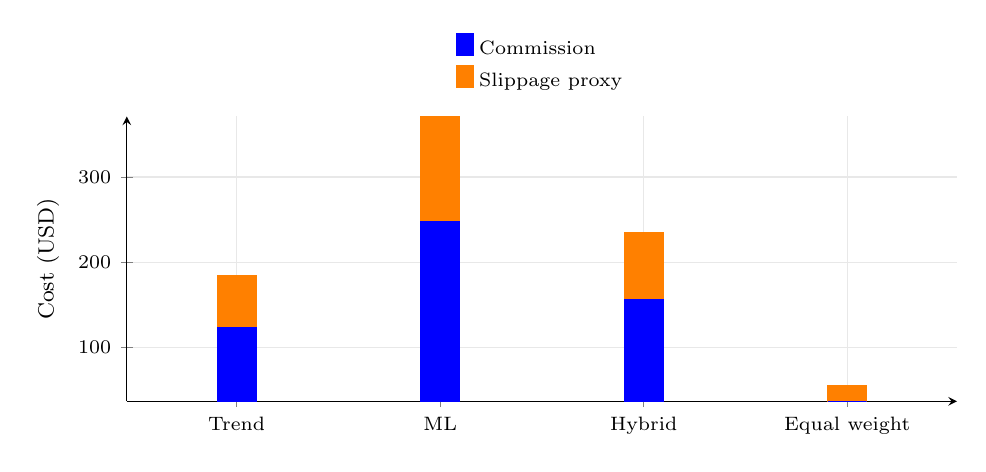
\begin{tikzpicture}
\begin{axis}[width=\linewidth,height=5.2cm,xtick={0,1,2,3},xticklabels={Trend,ML,Hybrid,Equal weight},enlarge x limits=.18,ybar stacked,bar width=14pt,ylabel={Cost (USD)},legend style={at={(.5,1.05)},anchor=south}]
\addplot+[blue] coordinates {(0,123.207203497) (1,247.34447747) (2,156.536969368) (3,37.1132402528)};
\addlegendentry{Commission}
\addplot+[orange] coordinates {(0,61.6036017484) (1,123.672238735) (2,78.2684846841) (3,18.5566201264)};
\addlegendentry{Slippage proxy}

\end{axis}
\end{tikzpicture}
\end{minipage}
\hfill
\begin{minipage}[t]{.48\linewidth}\centering
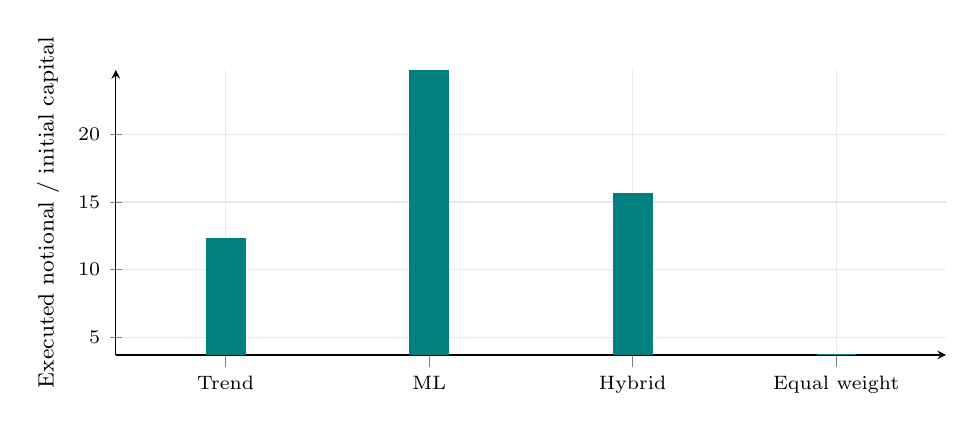
\begin{tikzpicture}
\begin{axis}[width=\linewidth,height=5.2cm,xtick={0,1,2,3},xticklabels={Trend,ML,Hybrid,Equal weight},enlarge x limits=.18,ybar,bar width=14pt,ylabel={Executed notional / initial capital}]
\addplot+[teal] coordinates {(0,12.3207203497) (1,24.734447747) (2,15.6536969368) (3,3.71132402528)};
\end{axis}
\end{tikzpicture}
\end{minipage}
\caption{Recorded exposure, turnover and cost diagnostics under the shared ledger contract.}\label{fig:11}
\end{figure}

Prediction loss and portfolio return need not rank models identically. The trading rule uses estimated payoff magnitude, abstention, weekly decisions and constrained capital. A prediction can be directionally wrong while its account is in cash; a correct signal can still lose after a delayed fill or costs. The decomposition therefore examines exposure, turnover, fill rejections, realized net outcomes and open holdings rather than attributing every equity change to classifier accuracy.

Over the full continuous hybrid account, modeled combined costs are 234.81 dollars across 2,541 fills. There are 1,367 sell fills, which include partial reductions rather than necessarily completed flat-to-flat episodes. Their net realized profit is 2,929.53 dollars; open holdings and unclosed costs still matter for total equity. The 86 completed position episodes have a 46.51\% win rate, materially different from the sell-fill statistic. Neither is a strategy's independent trade success probability. The completed-position episode table reconciles closed net profit and terminal open-position profit to total account profit, preventing partial sales from being counted as independent completed trades.

\noindent Table~\ref{tab:14} reports hybrid closed-position episodes versus still-open positions.

\begin{table}[!htbp]\centering\footnotesize\setlength{\tabcolsep}{3pt}\renewcommand{\arraystretch}{1.14}
\caption{Hybrid closed-position episodes versus still-open positions}\label{tab:14}
\begin{tabular}{@{}>{\raggedright\arraybackslash}p{\dimexpr 0.12303\textwidth-5.143pt\relax}>{\raggedleft\arraybackslash}p{\dimexpr 0.12303\textwidth-5.143pt\relax}>{\raggedleft\arraybackslash}p{\dimexpr 0.12303\textwidth-5.143pt\relax}>{\raggedleft\arraybackslash}p{\dimexpr 0.13880\textwidth-5.143pt\relax}>{\raggedleft\arraybackslash}p{\dimexpr 0.17666\textwidth-5.143pt\relax}>{\raggedleft\arraybackslash}p{\dimexpr 0.15142\textwidth-5.143pt\relax}>{\raggedleft\arraybackslash}p{\dimexpr 0.16404\textwidth-5.143pt\relax}@{}}
\toprule
\textbf{Period} & \textbf{Closed} & \textbf{Open} & \textbf{Closed wins} & \textbf{Closed P\&L (\$)} & \textbf{Open P\&L (\$)} & \textbf{Total P\&L (\$)} \\
\midrule
full & 86 & 18 & 46.51\% & 1605.17 & 1902.90 & 3508.07 \\
audit & 14 & 16 & 14.29\% & -141.85 & 96.14 & -45.71 \\
\bottomrule\end{tabular}\par\smallskip
\raggedright\textit{Source:} \path{data/research-v2/tables/diag_round_trip_summary.csv}.
\end{table}


\noindent Table~\ref{tab:15} reports largest audit hybrid forecast losses, selected by registered loss ranking.

\begin{table}[!htbp]\centering\footnotesize\setlength{\tabcolsep}{3pt}\renewcommand{\arraystretch}{1.14}
\caption{Largest audit hybrid forecast losses, selected by registered loss ranking}\label{tab:15}
\begin{tabular}{@{}>{\raggedright\arraybackslash}p{\dimexpr 0.13176\textwidth-5.000pt\relax}>{\raggedright\arraybackslash}p{\dimexpr 0.33784\textwidth-5.000pt\relax}>{\raggedright\arraybackslash}p{\dimexpr 0.13176\textwidth-5.000pt\relax}>{\raggedright\arraybackslash}p{\dimexpr 0.13176\textwidth-5.000pt\relax}>{\raggedleft\arraybackslash}p{\dimexpr 0.13514\textwidth-5.000pt\relax}>{\raggedleft\arraybackslash}p{\dimexpr 0.13176\textwidth-5.000pt\relax}@{}}
\toprule
\textbf{Symbol} & \textbf{Decision} & \textbf{Observed} & \textbf{Predicted} & \textbf{Confidence} & \textbf{Loss} \\
\midrule
TSLA & 2026-09-09 00:00:00+00:00 & FLAT & UP & 0.547 & 2.612 \\
TSLA & 2026-09-10 00:00:00+00:00 & FLAT & UP & 0.487 & 2.528 \\
GOOGL & 2026-07-30 00:00:00+00:00 & FLAT & UP & 0.468 & 2.321 \\
XLI & 2026-08-20 00:00:00+00:00 & DOWN & UP & 0.638 & 2.154 \\
DIA & 2026-08-12 00:00:00+00:00 & DOWN & FLAT & 0.514 & 2.113 \\
\bottomrule\end{tabular}\par\smallskip
\raggedright\textit{Source:} \path{data/research-v2/tables/diag_failures.csv}.
\end{table}


The reported failure cases follow registered selection rules: representative observations, the largest confident forecast errors and the largest adverse account contributions. They are not handpicked success stories. A loss concentration can reveal concentrated exposure or a difficult period, but explaining why a model produced a probability requires tracing its actual inputs and fitted state. Descriptive associations between a gate and losses are not causal gate benefits. Component and gate interventions provide the relevant controlled evidence.

Across the registered completed hybrid sensitivity scenarios, the lowest terminal return is -1.17\% in delay\_1; the highest is 0.93\% in reserve\_zero. These extrema are descriptive stress outcomes, not candidates selected for deployment. A rejected-order scenario can improve a realized sample by avoiding losing exposure, and a temporary gap can worsen drawdown without changing the terminal price. Both effects require examining the full path, fills and rejections, not just ending wealth.

\noindent Table~\ref{tab:16} reports hybrid execution and risk sensitivities; fresh-capital audit.

\begin{table}[!htbp]\centering\footnotesize\setlength{\tabcolsep}{3pt}\renewcommand{\arraystretch}{1.14}
\caption{Hybrid execution and risk sensitivities; fresh-capital audit}\label{tab:16}
\begin{tabular}{@{}>{\raggedright\arraybackslash}p{\dimexpr 0.20189\textwidth-5.000pt\relax}>{\raggedright\arraybackslash}p{\dimexpr 0.30284\textwidth-5.000pt\relax}>{\raggedleft\arraybackslash}p{\dimexpr 0.12618\textwidth-5.000pt\relax}>{\raggedleft\arraybackslash}p{\dimexpr 0.12303\textwidth-5.000pt\relax}>{\raggedleft\arraybackslash}p{\dimexpr 0.12303\textwidth-5.000pt\relax}>{\raggedleft\arraybackslash}p{\dimexpr 0.12303\textwidth-5.000pt\relax}@{}}
\toprule
\textbf{Scenario} & \textbf{Status} & \textbf{Net return} & \textbf{Max DD} & \textbf{Fills} & \textbf{Rejected} \\
\midrule
base & completed & -0.46\% & -2.21\% & 217 & 6 \\
cost\_\allowbreak{}zero & completed & -0.25\% & -2.17\% & 217 & 6 \\
cost\_\allowbreak{}2x & completed & -0.66\% & -2.26\% & 217 & 6 \\
cost\_\allowbreak{}4x & completed & -1.07\% & -2.35\% & 217 & 6 \\
delay\_\allowbreak{}1 & completed & -1.17\% & -2.29\% & 219 & 4 \\
liquidity\_\allowbreak{}50pct & completed & -0.35\% & -2.22\% & 1,043 & 25 \\
gap\_\allowbreak{}down\_\allowbreak{}10pct & completed & -0.46\% & -6.45\% & 217 & 6 \\
risk\_\allowbreak{}gross\_\allowbreak{}60pct & completed & -0.47\% & -2.09\% & 213 & 7 \\
reserve\_\allowbreak{}zero & completed & 0.93\% & -2.09\% & 151 & 70 \\
missing\_\allowbreak{}bar & expected\_\allowbreak{}validation\_\allowbreak{}halt & - & - & - & - \\
\bottomrule\end{tabular}\par\smallskip
\raggedright\textit{Source:} \path{data/research-v2/tables/diag_stress.csv}.
\end{table}


\noindent Figure~\ref{fig:12} shows registered execution sensitivities; terminal return and path risk answer different questions.

\begin{figure}[htbp]\centering
% Native editable figure; frozen statistics 0d291b4aebf8c524dc6705d872c070feb990e86a1cebbd59a758f400b240c952
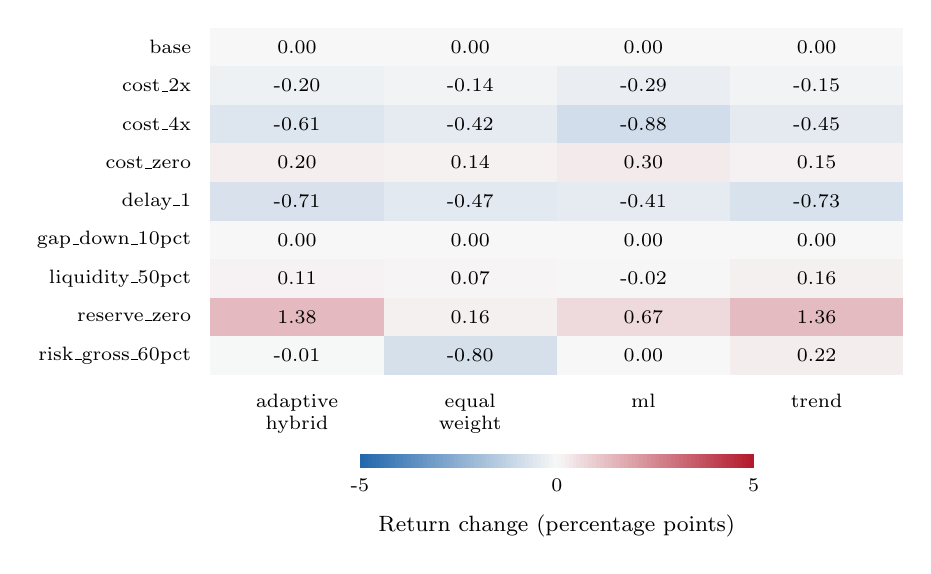
\begin{tikzpicture}[x=1cm,y=1cm,font=\scriptsize]
\node[anchor=east] at (-.12,4.165) {base};
\fill[fill={rgb,255:red,247;green,247;blue,247}] (0,3.92) rectangle ++(2.2,0.49);
\node at (1.1,4.165) {0.00};
\fill[fill={rgb,255:red,247;green,247;blue,247}] (2.2,3.92) rectangle ++(2.2,0.49);
\node at (3.3,4.165) {0.00};
\fill[fill={rgb,255:red,247;green,247;blue,247}] (4.4,3.92) rectangle ++(2.2,0.49);
\node at (5.5,4.165) {0.00};
\fill[fill={rgb,255:red,247;green,247;blue,247}] (6.6,3.92) rectangle ++(2.2,0.49);
\node at (7.7,4.165) {0.00};
\node[anchor=east] at (-.12,3.675) {cost\_2x};
\fill[fill={rgb,255:red,238;green,241;blue,244}] (0,3.43) rectangle ++(2.2,0.49);
\node at (1.1,3.675) {-0.20};
\fill[fill={rgb,255:red,241;green,243;blue,245}] (2.2,3.43) rectangle ++(2.2,0.49);
\node at (3.3,3.675) {-0.14};
\fill[fill={rgb,255:red,234;green,238;blue,243}] (4.4,3.43) rectangle ++(2.2,0.49);
\node at (5.5,3.675) {-0.29};
\fill[fill={rgb,255:red,241;green,243;blue,245}] (6.6,3.43) rectangle ++(2.2,0.49);
\node at (7.7,3.675) {-0.15};
\node[anchor=east] at (-.12,3.185) {cost\_4x};
\fill[fill={rgb,255:red,221;green,229;blue,238}] (0,2.94) rectangle ++(2.2,0.49);
\node at (1.1,3.185) {-0.61};
\fill[fill={rgb,255:red,229;green,235;blue,241}] (2.2,2.94) rectangle ++(2.2,0.49);
\node at (3.3,3.185) {-0.42};
\fill[fill={rgb,255:red,209;green,221;blue,234}] (4.4,2.94) rectangle ++(2.2,0.49);
\node at (5.5,3.185) {-0.88};
\fill[fill={rgb,255:red,228;green,234;blue,240}] (6.6,2.94) rectangle ++(2.2,0.49);
\node at (7.7,3.185) {-0.45};
\node[anchor=east] at (-.12,2.695) {cost\_zero};
\fill[fill={rgb,255:red,244;green,238;blue,239}] (0,2.45) rectangle ++(2.2,0.49);
\node at (1.1,2.695) {0.20};
\fill[fill={rgb,255:red,245;green,241;blue,241}] (2.2,2.45) rectangle ++(2.2,0.49);
\node at (3.3,2.695) {0.14};
\fill[fill={rgb,255:red,243;green,234;blue,235}] (4.4,2.45) rectangle ++(2.2,0.49);
\node at (5.5,2.695) {0.30};
\fill[fill={rgb,255:red,245;green,240;blue,241}] (6.6,2.45) rectangle ++(2.2,0.49);
\node at (7.7,2.695) {0.15};
\node[anchor=east] at (-.12,2.205) {delay\_1};
\fill[fill={rgb,255:red,217;green,226;blue,236}] (0,1.96) rectangle ++(2.2,0.49);
\node at (1.1,2.205) {-0.71};
\fill[fill={rgb,255:red,227;green,233;blue,240}] (2.2,1.96) rectangle ++(2.2,0.49);
\node at (3.3,2.205) {-0.47};
\fill[fill={rgb,255:red,229;green,235;blue,241}] (4.4,1.96) rectangle ++(2.2,0.49);
\node at (5.5,2.205) {-0.41};
\fill[fill={rgb,255:red,216;green,226;blue,236}] (6.6,1.96) rectangle ++(2.2,0.49);
\node at (7.7,2.205) {-0.73};
\node[anchor=east] at (-.12,1.715) {gap\_down\_10pct};
\fill[fill={rgb,255:red,247;green,247;blue,247}] (0,1.47) rectangle ++(2.2,0.49);
\node at (1.1,1.715) {0.00};
\fill[fill={rgb,255:red,247;green,247;blue,247}] (2.2,1.47) rectangle ++(2.2,0.49);
\node at (3.3,1.715) {0.00};
\fill[fill={rgb,255:red,247;green,247;blue,247}] (4.4,1.47) rectangle ++(2.2,0.49);
\node at (5.5,1.715) {0.00};
\fill[fill={rgb,255:red,247;green,247;blue,247}] (6.6,1.47) rectangle ++(2.2,0.49);
\node at (7.7,1.715) {0.00};
\node[anchor=east] at (-.12,1.225) {liquidity\_50pct};
\fill[fill={rgb,255:red,246;green,242;blue,243}] (0,0.98) rectangle ++(2.2,0.49);
\node at (1.1,1.225) {0.11};
\fill[fill={rgb,255:red,246;green,244;blue,244}] (2.2,0.98) rectangle ++(2.2,0.49);
\node at (3.3,1.225) {0.07};
\fill[fill={rgb,255:red,246;green,246;blue,247}] (4.4,0.98) rectangle ++(2.2,0.49);
\node at (5.5,1.225) {-0.02};
\fill[fill={rgb,255:red,245;green,240;blue,240}] (6.6,0.98) rectangle ++(2.2,0.49);
\node at (7.7,1.225) {0.16};
\node[anchor=east] at (-.12,0.735) {reserve\_zero};
\fill[fill={rgb,255:red,228;green,185;blue,191}] (0,0.49) rectangle ++(2.2,0.49);
\node at (1.1,0.735) {1.38};
\fill[fill={rgb,255:red,245;green,240;blue,240}] (2.2,0.49) rectangle ++(2.2,0.49);
\node at (3.3,0.735) {0.16};
\fill[fill={rgb,255:red,238;green,217;blue,220}] (4.4,0.49) rectangle ++(2.2,0.49);
\node at (5.5,0.735) {0.67};
\fill[fill={rgb,255:red,228;green,187;blue,192}] (6.6,0.49) rectangle ++(2.2,0.49);
\node at (7.7,0.735) {1.36};
\node[anchor=east] at (-.12,0.245) {risk\_gross\_60pct};
\fill[fill={rgb,255:red,246;green,247;blue,247}] (0,0) rectangle ++(2.2,0.49);
\node at (1.1,0.245) {-0.01};
\fill[fill={rgb,255:red,213;green,224;blue,235}] (2.2,0) rectangle ++(2.2,0.49);
\node at (3.3,0.245) {-0.80};
\fill[fill={rgb,255:red,247;green,247;blue,247}] (4.4,0) rectangle ++(2.2,0.49);
\node at (5.5,0.245) {0.00};
\fill[fill={rgb,255:red,244;green,237;blue,238}] (6.6,0) rectangle ++(2.2,0.49);
\node at (7.7,0.245) {0.22};
\node[anchor=north,align=center] at (1.1,-.12) {adaptive\\hybrid};
\node[anchor=north,align=center] at (3.3,-.12) {equal\\weight};
\node[anchor=north,align=center] at (5.5,-.12) {ml};
\node[anchor=north,align=center] at (7.7,-.12) {trend};
\fill[fill={rgb,255:red,35;green,103;blue,173}] (1.9,-1.18) rectangle ++(.051,.18);
\fill[fill={rgb,255:red,39;green,106;blue,174}] (1.95,-1.18) rectangle ++(.051,.18);
\fill[fill={rgb,255:red,44;green,109;blue,176}] (2,-1.18) rectangle ++(.051,.18);
\fill[fill={rgb,255:red,48;green,112;blue,177}] (2.05,-1.18) rectangle ++(.051,.18);
\fill[fill={rgb,255:red,52;green,115;blue,179}] (2.1,-1.18) rectangle ++(.051,.18);
\fill[fill={rgb,255:red,57;green,118;blue,180}] (2.15,-1.18) rectangle ++(.051,.18);
\fill[fill={rgb,255:red,61;green,121;blue,182}] (2.2,-1.18) rectangle ++(.051,.18);
\fill[fill={rgb,255:red,65;green,124;blue,183}] (2.25,-1.18) rectangle ++(.051,.18);
\fill[fill={rgb,255:red,69;green,127;blue,185}] (2.3,-1.18) rectangle ++(.051,.18);
\fill[fill={rgb,255:red,74;green,130;blue,186}] (2.35,-1.18) rectangle ++(.051,.18);
\fill[fill={rgb,255:red,78;green,132;blue,188}] (2.4,-1.18) rectangle ++(.051,.18);
\fill[fill={rgb,255:red,82;green,135;blue,189}] (2.45,-1.18) rectangle ++(.051,.18);
\fill[fill={rgb,255:red,86;green,138;blue,191}] (2.5,-1.18) rectangle ++(.051,.18);
\fill[fill={rgb,255:red,91;green,141;blue,192}] (2.55,-1.18) rectangle ++(.051,.18);
\fill[fill={rgb,255:red,95;green,144;blue,194}] (2.6,-1.18) rectangle ++(.051,.18);
\fill[fill={rgb,255:red,99;green,147;blue,195}] (2.65,-1.18) rectangle ++(.051,.18);
\fill[fill={rgb,255:red,104;green,150;blue,197}] (2.7,-1.18) rectangle ++(.051,.18);
\fill[fill={rgb,255:red,108;green,153;blue,198}] (2.75,-1.18) rectangle ++(.051,.18);
\fill[fill={rgb,255:red,112;green,156;blue,200}] (2.8,-1.18) rectangle ++(.051,.18);
\fill[fill={rgb,255:red,116;green,159;blue,201}] (2.85,-1.18) rectangle ++(.051,.18);
\fill[fill={rgb,255:red,121;green,161;blue,203}] (2.9,-1.18) rectangle ++(.051,.18);
\fill[fill={rgb,255:red,125;green,164;blue,204}] (2.95,-1.18) rectangle ++(.051,.18);
\fill[fill={rgb,255:red,129;green,167;blue,206}] (3,-1.18) rectangle ++(.051,.18);
\fill[fill={rgb,255:red,134;green,170;blue,207}] (3.05,-1.18) rectangle ++(.051,.18);
\fill[fill={rgb,255:red,138;green,173;blue,209}] (3.1,-1.18) rectangle ++(.051,.18);
\fill[fill={rgb,255:red,142;green,176;blue,210}] (3.15,-1.18) rectangle ++(.051,.18);
\fill[fill={rgb,255:red,146;green,179;blue,212}] (3.2,-1.18) rectangle ++(.051,.18);
\fill[fill={rgb,255:red,151;green,182;blue,213}] (3.25,-1.18) rectangle ++(.051,.18);
\fill[fill={rgb,255:red,155;green,185;blue,215}] (3.3,-1.18) rectangle ++(.051,.18);
\fill[fill={rgb,255:red,159;green,188;blue,216}] (3.35,-1.18) rectangle ++(.051,.18);
\fill[fill={rgb,255:red,164;green,190;blue,218}] (3.4,-1.18) rectangle ++(.051,.18);
\fill[fill={rgb,255:red,168;green,193;blue,219}] (3.45,-1.18) rectangle ++(.051,.18);
\fill[fill={rgb,255:red,172;green,196;blue,221}] (3.5,-1.18) rectangle ++(.051,.18);
\fill[fill={rgb,255:red,176;green,199;blue,222}] (3.55,-1.18) rectangle ++(.051,.18);
\fill[fill={rgb,255:red,181;green,202;blue,224}] (3.6,-1.18) rectangle ++(.051,.18);
\fill[fill={rgb,255:red,185;green,205;blue,225}] (3.65,-1.18) rectangle ++(.051,.18);
\fill[fill={rgb,255:red,189;green,208;blue,227}] (3.7,-1.18) rectangle ++(.051,.18);
\fill[fill={rgb,255:red,194;green,211;blue,228}] (3.75,-1.18) rectangle ++(.051,.18);
\fill[fill={rgb,255:red,198;green,214;blue,230}] (3.8,-1.18) rectangle ++(.051,.18);
\fill[fill={rgb,255:red,202;green,217;blue,231}] (3.85,-1.18) rectangle ++(.051,.18);
\fill[fill={rgb,255:red,206;green,219;blue,233}] (3.9,-1.18) rectangle ++(.051,.18);
\fill[fill={rgb,255:red,211;green,222;blue,234}] (3.95,-1.18) rectangle ++(.051,.18);
\fill[fill={rgb,255:red,215;green,225;blue,236}] (4,-1.18) rectangle ++(.051,.18);
\fill[fill={rgb,255:red,219;green,228;blue,237}] (4.05,-1.18) rectangle ++(.051,.18);
\fill[fill={rgb,255:red,223;green,231;blue,239}] (4.1,-1.18) rectangle ++(.051,.18);
\fill[fill={rgb,255:red,228;green,234;blue,240}] (4.15,-1.18) rectangle ++(.051,.18);
\fill[fill={rgb,255:red,232;green,237;blue,242}] (4.2,-1.18) rectangle ++(.051,.18);
\fill[fill={rgb,255:red,236;green,240;blue,243}] (4.25,-1.18) rectangle ++(.051,.18);
\fill[fill={rgb,255:red,241;green,243;blue,245}] (4.3,-1.18) rectangle ++(.051,.18);
\fill[fill={rgb,255:red,245;green,246;blue,246}] (4.35,-1.18) rectangle ++(.051,.18);
\fill[fill={rgb,255:red,246;green,245;blue,245}] (4.4,-1.18) rectangle ++(.051,.18);
\fill[fill={rgb,255:red,245;green,240;blue,241}] (4.45,-1.18) rectangle ++(.051,.18);
\fill[fill={rgb,255:red,244;green,236;blue,237}] (4.5,-1.18) rectangle ++(.051,.18);
\fill[fill={rgb,255:red,242;green,231;blue,233}] (4.55,-1.18) rectangle ++(.051,.18);
\fill[fill={rgb,255:red,241;green,227;blue,229}] (4.6,-1.18) rectangle ++(.051,.18);
\fill[fill={rgb,255:red,239;green,222;blue,225}] (4.65,-1.18) rectangle ++(.051,.18);
\fill[fill={rgb,255:red,238;green,218;blue,220}] (4.7,-1.18) rectangle ++(.051,.18);
\fill[fill={rgb,255:red,237;green,214;blue,216}] (4.75,-1.18) rectangle ++(.051,.18);
\fill[fill={rgb,255:red,235;green,209;blue,212}] (4.8,-1.18) rectangle ++(.051,.18);
\fill[fill={rgb,255:red,234;green,205;blue,208}] (4.85,-1.18) rectangle ++(.051,.18);
\fill[fill={rgb,255:red,233;green,200;blue,204}] (4.9,-1.18) rectangle ++(.051,.18);
\fill[fill={rgb,255:red,231;green,196;blue,200}] (4.95,-1.18) rectangle ++(.051,.18);
\fill[fill={rgb,255:red,230;green,191;blue,196}] (5,-1.18) rectangle ++(.051,.18);
\fill[fill={rgb,255:red,228;green,187;blue,192}] (5.05,-1.18) rectangle ++(.051,.18);
\fill[fill={rgb,255:red,227;green,182;blue,188}] (5.1,-1.18) rectangle ++(.051,.18);
\fill[fill={rgb,255:red,226;green,178;blue,184}] (5.15,-1.18) rectangle ++(.051,.18);
\fill[fill={rgb,255:red,224;green,173;blue,180}] (5.2,-1.18) rectangle ++(.051,.18);
\fill[fill={rgb,255:red,223;green,169;blue,176}] (5.25,-1.18) rectangle ++(.051,.18);
\fill[fill={rgb,255:red,221;green,164;blue,172}] (5.3,-1.18) rectangle ++(.051,.18);
\fill[fill={rgb,255:red,220;green,160;blue,167}] (5.35,-1.18) rectangle ++(.051,.18);
\fill[fill={rgb,255:red,219;green,156;blue,163}] (5.4,-1.18) rectangle ++(.051,.18);
\fill[fill={rgb,255:red,217;green,151;blue,159}] (5.45,-1.18) rectangle ++(.051,.18);
\fill[fill={rgb,255:red,216;green,147;blue,155}] (5.5,-1.18) rectangle ++(.051,.18);
\fill[fill={rgb,255:red,215;green,142;blue,151}] (5.55,-1.18) rectangle ++(.051,.18);
\fill[fill={rgb,255:red,213;green,138;blue,147}] (5.6,-1.18) rectangle ++(.051,.18);
\fill[fill={rgb,255:red,212;green,133;blue,143}] (5.65,-1.18) rectangle ++(.051,.18);
\fill[fill={rgb,255:red,210;green,129;blue,139}] (5.7,-1.18) rectangle ++(.051,.18);
\fill[fill={rgb,255:red,209;green,124;blue,135}] (5.75,-1.18) rectangle ++(.051,.18);
\fill[fill={rgb,255:red,208;green,120;blue,131}] (5.8,-1.18) rectangle ++(.051,.18);
\fill[fill={rgb,255:red,206;green,115;blue,127}] (5.85,-1.18) rectangle ++(.051,.18);
\fill[fill={rgb,255:red,205;green,111;blue,123}] (5.9,-1.18) rectangle ++(.051,.18);
\fill[fill={rgb,255:red,204;green,107;blue,118}] (5.95,-1.18) rectangle ++(.051,.18);
\fill[fill={rgb,255:red,202;green,102;blue,114}] (6,-1.18) rectangle ++(.051,.18);
\fill[fill={rgb,255:red,201;green,98;blue,110}] (6.05,-1.18) rectangle ++(.051,.18);
\fill[fill={rgb,255:red,199;green,93;blue,106}] (6.1,-1.18) rectangle ++(.051,.18);
\fill[fill={rgb,255:red,198;green,89;blue,102}] (6.15,-1.18) rectangle ++(.051,.18);
\fill[fill={rgb,255:red,197;green,84;blue,98}] (6.2,-1.18) rectangle ++(.051,.18);
\fill[fill={rgb,255:red,195;green,80;blue,94}] (6.25,-1.18) rectangle ++(.051,.18);
\fill[fill={rgb,255:red,194;green,75;blue,90}] (6.3,-1.18) rectangle ++(.051,.18);
\fill[fill={rgb,255:red,192;green,71;blue,86}] (6.35,-1.18) rectangle ++(.051,.18);
\fill[fill={rgb,255:red,191;green,66;blue,82}] (6.4,-1.18) rectangle ++(.051,.18);
\fill[fill={rgb,255:red,190;green,62;blue,78}] (6.45,-1.18) rectangle ++(.051,.18);
\fill[fill={rgb,255:red,188;green,57;blue,74}] (6.5,-1.18) rectangle ++(.051,.18);
\fill[fill={rgb,255:red,187;green,53;blue,70}] (6.55,-1.18) rectangle ++(.051,.18);
\fill[fill={rgb,255:red,186;green,49;blue,65}] (6.6,-1.18) rectangle ++(.051,.18);
\fill[fill={rgb,255:red,184;green,44;blue,61}] (6.65,-1.18) rectangle ++(.051,.18);
\fill[fill={rgb,255:red,183;green,40;blue,57}] (6.7,-1.18) rectangle ++(.051,.18);
\fill[fill={rgb,255:red,181;green,35;blue,53}] (6.75,-1.18) rectangle ++(.051,.18);
\fill[fill={rgb,255:red,180;green,31;blue,49}] (6.8,-1.18) rectangle ++(.051,.18);
\fill[fill={rgb,255:red,179;green,26;blue,45}] (6.85,-1.18) rectangle ++(.051,.18);
\node[anchor=north] at (1.9,-1.2) {-5};
\node[anchor=north] at (4.4,-1.2) {0};
\node[anchor=north] at (6.9,-1.2) {5};
\node[anchor=north,font=\footnotesize] at (4.4,-1.65) {Return change (percentage points)};
\end{tikzpicture}
\caption{Registered execution sensitivities; terminal return and path risk answer different questions.}\label{fig:12}
\end{figure}

The simulator's costs are assumptions rather than measured execution. Fixed proportional slippage cannot represent all auction impact, spreads, illiquidity or market halts. Bounded fill scenarios explore one aspect of capacity without certifying real fill quality. A small simulated account may reduce some capacity concerns, but that does not make every close executable at the modeled price. Broker deployment would require timing, corporate-action and reconciliation evidence that this study deliberately does not claim.

\section{Operational evaluation and prospective collection}\label{sec:section-09}

The active r2 runtime passed 27 source-bound tests. All 8 actual process-kill checkpoints recovered with equivalent state, and 5 altered-release evidence cases were refused. The operating system invoked the frozen command at 2026-09-28T08:50:56.358915+00:00; its parent PID was 1. That commissioning run validated 22 instruments, prepared signals and targets, persisted both accounts and reconciled them. Its receipt was then restored at the registered original path while preserving the prior directory. Commissioning is isolated from the pilot: the verified observed decision count is 0, mature count 0, and terminal mark count 0. The schedule's next event is 2026-09-30T04:30:00+08:00 Hong Kong. No remote trading workflow was executed; the inspected GitHub workflow was disabled by inactivity. Physical sleep/power-loss and sustained session-close availability remain unobserved.

The actual cold provider-to-ledger commissioning took 33.27 seconds, including 30.11 seconds of public-data reads. It made 22 requests with 0 observed provider failures. Across 20 warm batches, median batch time was 1.798 seconds and empirical P95 was 4.159 seconds. A separate 5-fit SPY timing sample had median 0.424 seconds. Cold-run and small training samples do not support tail-latency estimates; warm P95 is descriptive. The collector ran on the recorded arm64 macOS host under concurrent research load.

\noindent Table~\ref{tab:17} reports warm pipeline stage timings, seconds; P99 intentionally unreported.

\begin{table}[!htbp]\centering\footnotesize\setlength{\tabcolsep}{3pt}\renewcommand{\arraystretch}{1.14}
\caption{Warm pipeline stage timings, seconds; P99 intentionally unreported}\label{tab:17}
\begin{tabular}{@{}>{\raggedright\arraybackslash}p{\dimexpr 0.22000\textwidth-4.800pt\relax}>{\raggedleft\arraybackslash}p{\dimexpr 0.19500\textwidth-4.800pt\relax}>{\raggedleft\arraybackslash}p{\dimexpr 0.19500\textwidth-4.800pt\relax}>{\raggedleft\arraybackslash}p{\dimexpr 0.19500\textwidth-4.800pt\relax}>{\raggedleft\arraybackslash}p{\dimexpr 0.19500\textwidth-4.800pt\relax}@{}}
\toprule
\textbf{Stage} & \textbf{Samples} & \textbf{P50 (s)} & \textbf{P95 (s)} & \textbf{P99 (s)} \\
\midrule
features & 20 & 0.372 & 1.083 & - \\
inference & 20 & 0.191 & 0.354 & - \\
whole\_\allowbreak{}batch & 20 & 1.798 & 4.159 & - \\
\bottomrule\end{tabular}\par\smallskip
\raggedright\textit{Source:} \path{data/research-v2/operations/latency-r2.json}.
\end{table}


\noindent Table~\ref{tab:18} reports actual verification jobs; overlapping suites are separate records.

\begin{table}[!htbp]\centering\footnotesize\setlength{\tabcolsep}{3pt}\renewcommand{\arraystretch}{1.14}
\caption{Actual verification jobs; overlapping suites are separate records}\label{tab:18}
\begin{tabular}{@{}>{\raggedright\arraybackslash}p{\dimexpr 0.56180\textwidth-4.800pt\relax}>{\raggedleft\arraybackslash}p{\dimexpr 0.10955\textwidth-4.800pt\relax}>{\raggedleft\arraybackslash}p{\dimexpr 0.10955\textwidth-4.800pt\relax}>{\raggedleft\arraybackslash}p{\dimexpr 0.10955\textwidth-4.800pt\relax}>{\raggedleft\arraybackslash}p{\dimexpr 0.10955\textwidth-4.800pt\relax}@{}}
\toprule
\textbf{Saved report} & \textbf{Cases} & \textbf{Failed} & \textbf{Errors} & \textbf{Skipped} \\
\midrule
data/\allowbreak{}research-v2/\allowbreak{}tests/\allowbreak{}baseline-offline.xml & 310 & 0 & 0 & 0 \\
data/\allowbreak{}research-v2/\allowbreak{}tests/\allowbreak{}final-offline/\allowbreak{}results.xml & 370 & 0 & 0 & 0 \\
data/\allowbreak{}research-v2/\allowbreak{}tests/\allowbreak{}final-qualified/\allowbreak{}results.xml & 370 & 0 & 0 & 0 \\
data/\allowbreak{}research-v2/\allowbreak{}tests/\allowbreak{}final-stable/\allowbreak{}results.xml & 370 & 0 & 0 & 0 \\
data/\allowbreak{}research-v2/\allowbreak{}tests/\allowbreak{}provider-integration.xml & 17 & 0 & 0 & 0 \\
data/\allowbreak{}research-v2/\allowbreak{}tests/\allowbreak{}ui-integration.xml & 1 & 0 & 0 & 0 \\
data/\allowbreak{}research-v2/\allowbreak{}tests/\allowbreak{}ui-r2/\allowbreak{}results.xml & 1 & 0 & 0 & 0 \\
data/\allowbreak{}research-v2/\allowbreak{}tests/\allowbreak{}ui-r2-qualified/\allowbreak{}results.xml & 1 & 0 & 0 & 0 \\
\bottomrule\end{tabular}\par\smallskip
\raggedright\textit{Source:} \path{data/research-v2/tests/*.xml; XML testcase counts}.
\end{table}


\noindent Figure~\ref{fig:13} shows measured fitting latency by registered variant under differing run order and concurrent host load; these are operational timings, not controlled speedup estimates.

\begin{figure}[htbp]\centering
% Native editable figure; frozen statistics 0d291b4aebf8c524dc6705d872c070feb990e86a1cebbd59a758f400b240c952
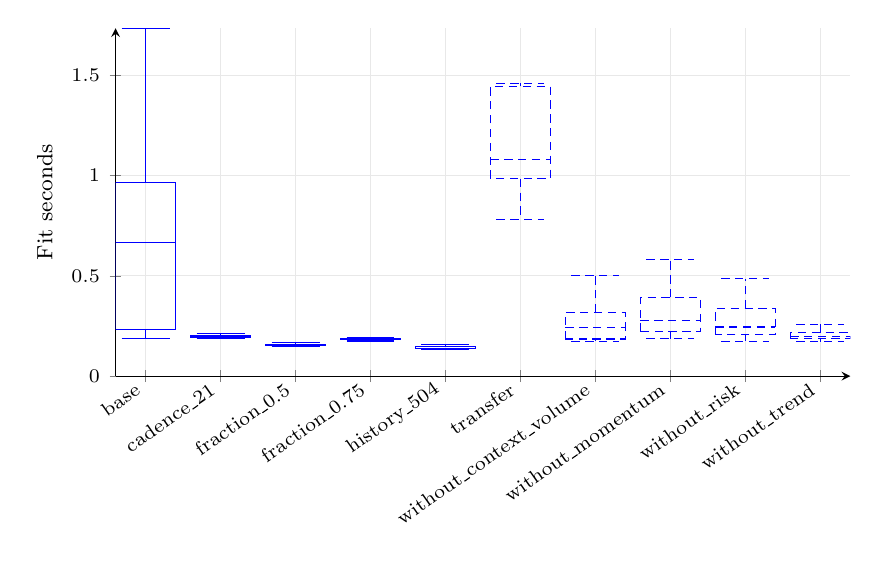
\begin{tikzpicture}
\begin{axis}[width=.9\linewidth,height=6cm,boxplot/draw direction=y,xtick={0,1,2,3,4,5,6,7,8,9},xticklabels={{base},{cadence\_21},{fraction\_0.5},{fraction\_0.75},{history\_504},{transfer},{without\_context\_volume},{without\_momentum},{without\_risk},{without\_trend}},x tick label style={rotate=35,anchor=east},ylabel={Fit seconds},ymin=0]
\addplot+[boxplot prepared={draw position=0,lower whisker=0.187755082996,lower quartile=0.230702500245,median=0.667628895499,upper quartile=0.966208124744,upper whisker=1.733549875},blue] coordinates {};
\addplot+[boxplot prepared={draw position=1,lower whisker=0.187187374991,lower quartile=0.192843219254,median=0.197883166991,upper quartile=0.201251249491,upper whisker=0.212719375006},blue] coordinates {};
\addplot+[boxplot prepared={draw position=2,lower whisker=0.145877624993,lower quartile=0.152505896251,median=0.155188041506,upper quartile=0.158791937243,upper whisker=0.166472625002},blue] coordinates {};
\addplot+[boxplot prepared={draw position=3,lower whisker=0.174998332994,lower quartile=0.181211584,median=0.184082833497,upper quartile=0.185834291995,upper whisker=0.191644124992},blue] coordinates {};
\addplot+[boxplot prepared={draw position=4,lower whisker=0.133230000007,lower quartile=0.137934395501,median=0.1396283125,upper quartile=0.147123426996,upper whisker=0.157956458992},blue] coordinates {};
\addplot+[boxplot prepared={draw position=5,lower whisker=0.779778124997,lower quartile=0.983922364248,median=1.07975004199,upper quartile=1.443187437,upper whisker=1.45833337501},blue] coordinates {};
\addplot+[boxplot prepared={draw position=6,lower whisker=0.174084333994,lower quartile=0.18489948925,median=0.241868416495,upper quartile=0.318596260506,upper whisker=0.500081375008},blue] coordinates {};
\addplot+[boxplot prepared={draw position=7,lower whisker=0.186025834002,lower quartile=0.22113709425,median=0.275304978997,upper quartile=0.392184739751,upper whisker=0.581473124999},blue] coordinates {};
\addplot+[boxplot prepared={draw position=8,lower whisker=0.174779500012,lower quartile=0.207700540999,median=0.244683541998,upper quartile=0.338147614493,upper whisker=0.484661540992},blue] coordinates {};
\addplot+[boxplot prepared={draw position=9,lower whisker=0.17080854201,lower quartile=0.185769979245,median=0.199566438001,upper quartile=0.216780635245,upper whisker=0.258316874999},blue] coordinates {};

\end{axis}
\end{tikzpicture}

\caption{Measured fitting latency by registered variant under differing run order and concurrent host load; these are operational timings, not controlled speedup estimates.}\label{fig:13}
\end{figure}

The local scheduler uses exchange-session events rather than a fixed Hong Kong clock. Standard close+30 occurs at different local times across US daylight-saving changes, and early-close sessions advance the event. Only an eligible transient failure permits the registered retries; deterministic integrity or risk failures halt. The watchdog checks for an absent receipt as well as an explicitly failed one. Pre-open checks do not create replacement strategy decisions. Weekly archival and milestone reviews assess coverage, latency, risk and protocol deviations without choosing winners from pilot returns.

The collector cannot execute while its host is asleep or unavailable. On recovery it must distinguish an overdue event from a legitimate current event, record missed coverage and refuse backfilled prospective decisions. A real launchd trigger receipt demonstrates that the operating system invoked the current runner and it reached its persistent state. It does not demonstrate a future session-close invocation, sustained host availability or an always-on service. Those are observations that must accumulate.

\noindent Table~\ref{tab:19} reports registered XNYS events and Hong Kong display times.

\begin{table}[!htbp]\centering\footnotesize\setlength{\tabcolsep}{3pt}\renewcommand{\arraystretch}{1.14}
\caption{Registered XNYS events and Hong Kong display times}\label{tab:19}
\begin{tabular}{@{}>{\raggedright\arraybackslash}p{\dimexpr 0.49153\textwidth-4.000pt\relax}>{\raggedleft\arraybackslash}p{\dimexpr 0.16949\textwidth-4.000pt\relax}>{\raggedright\arraybackslash}p{\dimexpr 0.33898\textwidth-4.000pt\relax}@{}}
\toprule
\textbf{Event} & \textbf{US session} & \textbf{Hong Kong trigger} \\
\midrule
Observed-session milestone 1 & 2026-09-29 & 2026-09-30 04:30 HKT \\
Observed-session milestone 5 & 2026-10-05 & 2026-10-06 04:30 HKT \\
Observed-session milestone 21 & 2026-10-27 & 2026-10-28 04:30 HKT \\
Observed-session milestone 42 & 2026-11-25 & 2026-11-26 05:30 HKT \\
Observed-session milestone 63 & 2026-12-28 & 2026-12-29 05:30 HKT \\
Model refit at anchor+21 & 2026-10-28 & 2026-10-29 04:30 HKT \\
Model refit at anchor+42 & 2026-11-27 & 2026-11-28 02:30 HKT \\
Final target-label endpoint & 2027-01-06 & 2027-01-07 05:30 HKT \\
\bottomrule\end{tabular}\par\smallskip
\raggedright\textit{Source:} \path{data/research-v2/tables/schedule_milestones.csv}.
\end{table}


The latest validated prospective analysis contains 0 decision receipts and 0 mature decision dates. It is recorded as interim. Commissioning, controlled replay and historical predictions are excluded from these counts. No prospective forecast or economic result is available; unobserved quantities are not zero returns or successful sessions.

Mature outcomes attach to earlier immutable decisions only after the execution-aligned endpoint is observed. After the final decision, six terminal sessions process outstanding fills and marks without generating new allocation targets. A halted account can still retain valid matured labels, but missing terminal accounting prevents a complete economic freeze. The read-only final-report command reconstructs the costed equal-weight comparator from those same observed snapshots and releases inferential results only at the registered final freeze; interim views are descriptive. The last decision date and the last label-maturity date are different. A missing expected session remains a recorded outage and does not shift the registered end until results become favorable. The operational observation period is not a promise of adequate power for a small economic effect. A strategy can complete the operational pilot and still fail the statistical or economic gate.

\section{Reproducibility and claim integrity}\label{sec:section-10}

The recorded test jobs are listed individually below; counts from separate or overlapping runs are not added into a fictional distinct-test total. Clean-environment reproduction evidence is retained in the source manifest and appendix. The complete clean replay retrained 848 trials (1,696 estimator fits), compared 352,800 forecast-view rows with maximum probability error 0.0e+00, and reproduced 40 portfolio histories covering 2,520 account sessions. Ledger states, targets, event lists, economic metrics and block-bootstrap/Holm outputs agreed. The comparison tolerances were rtol=1e-10 and atol=1e-12; actual probability error was zero. The sealed historical artifact comparison is distinct from the new clean-environment refits. Provider checks and UI commissioning are separate integration jobs with actual saved results.

The evidence package contains the protocol, exposure log, registry, per-trial configurations, saved predictions, fold boundaries, portfolio records, source tables and plot data. Original repaired experiments and sealed releases remain available. New results occupy versioned directories. The manuscript builder reads a single compiled statistics source and checks its inputs' hashes; generated empirical sentences and table cells carry source selectors in the claim map. A changed metric must update the dependent prose or fail validation. A missing figure source prevents a complete build.

Tests are recorded with command, runtime, collected test IDs, pass/fail/skip status and source hashes before and after execution. A passing JUnit file by itself cannot qualify unrelated source or an empty suite. Critical behavior includes mathematical accounting examples, future-data mutation, model serialization, release tampering, full-policy replay, concurrent execution, fault recovery and the dashboard-to-ledger path. Provider integration runs are explicitly separated from the default offline suite. Successful optional-provider checks do not admit those feeds into the primary model without historical eligibility evidence.

Clean-environment reproduction tests use the pinned core runtime and preserved artifacts. Byte-identical artifact checks, exact numeric comparisons and tolerance-based comparisons are separately named. This matters because serialized files may embed metadata even when numerical outputs agree. The package states what was actually rerun; it does not transform a saved verification claim into a new training run. Source inspection and local tests likewise do not certify a remote Actions deployment.

\section{Discussion and limitations}\label{sec:section-11}

The audit probability comparison has Holm-adjusted p=0.980 in its registered diagnostic family. The interval crosses zero, and the point estimate favors the prior. This combination supports a bounded statement: the current hybrid has not established better probability forecasts on the consumed audit. It does not prove exact equivalence, nor does it justify selecting a favorable instrument after inspecting the heatmap. The full registry retains the controlled follow-ups so that any narrower improvement is interpreted within its own dates, information set and uncertainty.

The most useful scientific distinction is between a weak forecasting result and an invalid experiment. Weak predictive or economic results remain publishable evidence when their design, uncertainty and limits are explicit. Conversely, stronger reported performance would not compensate for unavailable labels, inconsistent capital accounting or a search procedure hidden from the reader. This investigation makes those dependencies visible and creates a path for prospective replication without requiring the model to win.

Several limitations remain structural. The inherited universe has selection and survivorship bias. Current-vintage vendor adjustments do not reconstruct exactly what a historical participant saw. Overlapping ETFs and common market returns limit the independence of the cross section. Execution-aligned labels overlap in time. The short recent audit and finite development folds provide limited evidence across distinct regimes. Bootstrap intervals rely on local dependence assumptions and do not establish robustness to every structural break.

The controlled training budget is intentionally bounded. It evaluates a family of fixed, interpretable models rather than exhaustively searching all architectures. Excluding larger legacy models from a controlled table avoids an invalid comparison; it does not prove those models cannot work. A later architecture study would need its own registered information set, chronological partitions, compute budget and independent confirmation. Adding news or macro data would require actual availability evidence before any claim of incremental benefit.

Operational qualification also has a narrow scope. A local scheduler, persistent account and successful recovery test make collection feasible, but the user's host remains an availability dependency. Synthetic fault injection does not reproduce every filesystem or power-loss condition. The total-return proxy ledger omits real broker entitlements and market microstructure. No external orders are enabled, and no result here should be read as authorization for them. The deployment account remains cash unless independent evidence and separate execution gates eventually support a change.

\section{Conclusions}\label{sec:section-12}

The project now has a reproducible historical investigation and a separately versioned path for collecting prospective local evidence. On the recent audit, the calibrated mixture's 1.0882 log loss does not beat the prior's 1.0756; the capital-matched hybrid account also trails its simple investable control. Engineering tests and a real scheduler trigger support the tested collection contract, while sustained unattended sessions and final outcome maturity remain unobserved. The historical manuscript reports the available negative and mixed findings; the complete prospective study remains interim. No profitable-trader or broker-readiness approval follows from this work.

\clearpage\phantomsection\addcontentsline{toc}{section}{References}
\bibliographystyle{unsrtnat}
\bibliography{references}
\clearpage\appendix
\section{Complete instrument diagnostics}\label{sec:appendix-a}

\noindent Table~\ref{tab:20} reports complete audit instrument diagnostic for calibrated mixture.

\begin{table}[!htbp]\centering\footnotesize\setlength{\tabcolsep}{3pt}\renewcommand{\arraystretch}{1.14}
\caption{Complete audit instrument diagnostic for calibrated mixture}\label{tab:20}
\begin{tabular}{@{}>{\raggedright\arraybackslash}p{\dimexpr 0.16667\textwidth-5.000pt\relax}>{\raggedleft\arraybackslash}p{\dimexpr 0.16667\textwidth-5.000pt\relax}>{\raggedleft\arraybackslash}p{\dimexpr 0.16667\textwidth-5.000pt\relax}>{\raggedleft\arraybackslash}p{\dimexpr 0.16667\textwidth-5.000pt\relax}>{\raggedleft\arraybackslash}p{\dimexpr 0.16667\textwidth-5.000pt\relax}>{\raggedleft\arraybackslash}p{\dimexpr 0.16667\textwidth-5.000pt\relax}@{}}
\toprule
\textbf{Symbol} & \textbf{Rows} & \textbf{Accuracy} & \textbf{Balanced} & \textbf{Log loss} & \textbf{Brier} \\
\midrule
AAPL & 48 & 25.00\% & 33.33\% & 1.1004 & 0.6698 \\
AMZN & 48 & 54.17\% & 48.26\% & 1.0083 & 0.6010 \\
BAC & 48 & 37.50\% & 36.29\% & 1.0731 & 0.6505 \\
DIA & 48 & 47.92\% & 45.19\% & 1.0716 & 0.6453 \\
GLD & 48 & 33.33\% & 26.46\% & 1.1061 & 0.6716 \\
GOOGL & 48 & 50.00\% & 45.24\% & 1.0188 & 0.6137 \\
GS & 48 & 20.83\% & 33.33\% & 1.2844 & 0.7943 \\
IWM & 48 & 33.33\% & 29.63\% & 1.1020 & 0.6687 \\
JPM & 48 & 25.00\% & 28.25\% & 1.1186 & 0.6817 \\
META & 48 & 20.83\% & 16.83\% & 1.0474 & 0.6437 \\
MSFT & 48 & 37.50\% & 27.95\% & 1.0823 & 0.6691 \\
NVDA & 48 & 45.83\% & 32.96\% & 0.9877 & 0.6019 \\
QQQ & 48 & 43.75\% & 41.11\% & 1.0465 & 0.6301 \\
SPY & 48 & 35.42\% & 30.77\% & 1.0920 & 0.6642 \\
TLT & 48 & 52.08\% & 33.33\% & 1.0961 & 0.6459 \\
TSLA & 48 & 45.83\% & 26.63\% & 0.9251 & 0.5583 \\
XLE & 48 & 27.08\% & 27.47\% & 1.1033 & 0.6704 \\
XLF & 48 & 35.42\% & 31.44\% & 1.1115 & 0.6748 \\
XLI & 48 & 27.08\% & 37.04\% & 1.2959 & 0.7746 \\
XLK & 48 & 47.92\% & 36.95\% & 1.0659 & 0.6434 \\
XLP & 48 & 50.00\% & 37.33\% & 1.0604 & 0.6406 \\
XLV & 48 & 31.25\% & 35.43\% & 1.1420 & 0.6942 \\
\bottomrule\end{tabular}\par\smallskip
\raggedright\textit{Source:} \path{data/research-v2/tables/diag_instrument.csv}.
\end{table}


These rows use the same mature-label definition as the main analysis. Instrument rankings are descriptive and do not define a new selection policy. Machine-readable tables retain full precision, all registered variants and additional class/period slices omitted from the main text for readability.

\section{Fold, trial and evidence inventory}\label{sec:appendix-b}

\noindent Table~\ref{tab:21} reports question-to-evidence completion map.

\begingroup\footnotesize\setlength{\tabcolsep}{3pt}\renewcommand{\arraystretch}{1.14}
\begin{longtable}{@{}>{\raggedright\arraybackslash}p{\dimexpr 0.06555\textwidth-4.500pt\relax}>{\raggedright\arraybackslash}p{\dimexpr 0.16807\textwidth-4.500pt\relax}>{\raggedright\arraybackslash}p{\dimexpr 0.38319\textwidth-4.500pt\relax}>{\raggedright\arraybackslash}p{\dimexpr 0.38319\textwidth-4.500pt\relax}@{}}
\caption{Question-to-evidence completion map}\label{tab:21}\\
\toprule
\textbf{ID} & \textbf{Status} & \textbf{Evidence} & \textbf{Remaining limitation} \\
\midrule\endfirsthead
\multicolumn{4}{l}{\small\tablename\ \thetable\ (continued)}\\
\toprule
\textbf{ID} & \textbf{Status} & \textbf{Evidence} & \textbf{Remaining limitation} \\
\midrule\endhead
\midrule\multicolumn{4}{r}{\footnotesize Continued on the next page}\\\endfoot
\bottomrule\endlastfoot
R1 & verified with limitations & diag\_\allowbreak{}data\_\allowbreak{}coverage /\allowbreak{} dataset\_\allowbreak{}flow; snapshot hashes & Current-vintage prices; historical constituent/\allowbreak{}action tape unavailable \\
R2 & completed exploratory & diag\_\allowbreak{}forecast\_\allowbreak{}summary /\allowbreak{} paired\_\allowbreak{}inference; exp\_\allowbreak{}predictive & No independent historical confirmation; no edge approval \\
R3 & completed exploratory & diag\_\allowbreak{}calibration\_\allowbreak{}contrast; exp\_\allowbreak{}contrasts R3 & Separated gate benefit inconclusive \\
R4 & completed exploratory & exp\_\allowbreak{}predictive /\allowbreak{} portfolios /\allowbreak{} economic\_\allowbreak{}contrasts & Legacy larger models excluded from controlled comparisons \\
R5 & completed exploratory & exp\_\allowbreak{}contrasts R5; saved refit predictions & Family ablations are model-conditional, not causal mechanisms \\
R6 & completed exploratory & exp\_\allowbreak{}learning /\allowbreak{} model\_\allowbreak{}age /\allowbreak{} seeds & Bounded development-only budget; no pilot tuning \\
R7 & completed exploratory & diag\_\allowbreak{}instrument /\allowbreak{} regime; exp\_\allowbreak{}transfer & Held targets retain overlapping ETF economic exposures \\
R8 & completed exploratory & diag\_\allowbreak{}portfolio /\allowbreak{} round\_\allowbreak{}trip\_\allowbreak{}summary /\allowbreak{} total\_\allowbreak{}pnl\_\allowbreak{}attribution & Proxy fills and fixed proportional costs \\
R9 & completed exploratory & diag\_\allowbreak{}stress and replay ledgers & No closing-auction or empirical market-impact model \\
R10 & completed exploratory & diag\_\allowbreak{}failures /\allowbreak{} closed episodes /\allowbreak{} worst sell fills & Descriptive conditional evidence \\
R11 & tested local scope & Sealed runtime tests; scheduler-verification; UI and clean-env reports & Physical sleep/\allowbreak{}power-loss cycle and sustained availability unobserved \\
R12 & time-dependent & Registered63 sessions; active launchd; commissioning receipt & Independent sessions and final labels have not yet occurred \\
\end{longtable}
\noindent\textit{Source:} \path{data/research-v2/tables/evidence_matrix.csv}.\par\endgroup
\medskip


\noindent Table~\ref{tab:22} reports research-family registry status.

\begin{table}[!htbp]\centering\footnotesize\setlength{\tabcolsep}{3pt}\renewcommand{\arraystretch}{1.14}
\caption{Research-family registry status}\label{tab:22}
\begin{tabular}{@{}>{\raggedright\arraybackslash}p{\dimexpr 0.10744\textwidth-4.000pt\relax}>{\raggedright\arraybackslash}p{\dimexpr 0.62810\textwidth-4.000pt\relax}>{\raggedright\arraybackslash}p{\dimexpr 0.26446\textwidth-4.000pt\relax}@{}}
\toprule
\textbf{ID} & \textbf{Question} & \textbf{Recorded status} \\
\midrule
R1 & data provenance and accounting & completed\_\allowbreak{}exploratory \\
R2 & baselines and predictive value & completed\_\allowbreak{}exploratory \\
R3 & raw/\allowbreak{}calibrated and separated gating & completed\_\allowbreak{}exploratory \\
R4 & components/\allowbreak{}fixed mixture/\allowbreak{}adaptive gate & completed\_\allowbreak{}exploratory \\
R5 & feature family refits & completed\_\allowbreak{}exploratory \\
R6 & training fraction/\allowbreak{}history/\allowbreak{}cadence & completed\_\allowbreak{}exploratory \\
R7 & temporal and genuinely held-instrument transfer & completed\_\allowbreak{}exploratory \\
R8 & matched-capital economic performance & completed\_\allowbreak{}exploratory \\
R9 & cost/\allowbreak{}delay/\allowbreak{}missing-bar/\allowbreak{}gap/\allowbreak{}liquidity/\allowbreak{}risk sensitivity & completed\_\allowbreak{}exploratory \\
R10 & registered worst/\allowbreak{}confident-error and representative cases & completed\_\allowbreak{}exploratory \\
R11 & runtime/\allowbreak{}recovery/\allowbreak{}scheduler/\allowbreak{}full-policy parity & tested\_\allowbreak{}local\_\allowbreak{}scope \\
R12 & prospective replication & active\_\allowbreak{}awaiting\_\allowbreak{}evidence \\
\bottomrule\end{tabular}\par\smallskip
\raggedright\textit{Source:} \path{data/research-v2/registry/R*.json}.
\end{table}


R12 cannot be completed today: prospective decisions, operational coverage and execution-aligned outcome endpoints must occur in real time. The frozen first decision, final decision and final maturity events are listed in the schedule table. Missing sessions create deviations and a visible halt. Rebuilding this manuscript after observation requires refreshing the evidence snapshot, compiling statistics and rerunning the consistency checks.

\clearpage

\section{Reproduction commands and interpretation}\label{sec:appendix-c}

\begin{Verbatim}[breaklines=true,breakanywhere=true,fontsize=\scriptsize]
# From /Users/a/Downloads/ml-trade-engine
# Verify / inspect the frozen collector (read-only)
data/research-v2/clean-env/bin/python data/releases/research-v2-runtime-20260928-r2/scripts/collector_v2.py status --release data/releases/research-v2-runtime-20260928-r2 --workspace data/paper/research-v2
# Launch the product console
/Users/a/miniconda3/bin/python -m streamlit run app_v2.py --server.port 8504
# Recompute saved-data diagnostics under their recorded protocol
/Users/a/miniconda3/bin/python -B -m research_v2.diagnostics
# Resume registered controlled trials; completed checkpoints are verified
/Users/a/miniconda3/bin/python -B -m research_v2.experiments run
# Interim observed evidence (new output directory; never starts collection)
data/research-v2/clean-env/bin/python -B -m research_v2.prospective_report --output data/research-v2/prospective/NEW-DATED-RUN
# After all63 decisions and final six-session maturity only, add --freeze
# Compile checked statistics / editable manuscript
/Users/a/miniconda3/bin/python -B -m research_v2.paper compile
# Render PDF using bundled document runtime
/Users/a/.cache/codex-runtimes/codex-primary-runtime/dependencies/python/bin/python3 -B -m research_v2.paper pdf
\end{Verbatim}

Every command writes new evidence or reads a sealed artifact. Do not overwrite the existing release to conceal a changed method. Historical diagnostics can be regenerated immediately from the saved data. Prospective receipts and outcomes require the actual passage of exchange sessions, host availability and completed label endpoints. The historical manuscript can be substantively complete while the full prospective study remains interim.

\end{document}
